\subsection{Comparison of Prediction Methods}

EG01-EG23, EG01-EG24, EG01-EG29, and EG01-EG30 transition scenarios
are setup in \Cyclus using \deploy. 
To determine the most effective \deploy prediction methods, a
comparison of each prediction method for each 
transition scenario is conducted for both constant and 
linearly increasing power demand curves.
Similar to the simple transition scenario, these transition scenario 
simulations begin with an initial fleet of \glspl{LWR} 
that are progressively decommissioned starting at the 80 year mark, 
after which \deploy deploys \glspl{SFR} and \gls{MOX} \glspl{LWR} to meet 
the power demand. 
Figure \ref{fig:eg2329}
shows the setup of facilities and mass flows for 
EG01-23 and EG01-29 in \Cyclus. 
In EG01-23 and EG01-29, only plutonium is recycled from \gls{LWR}
spent fuel to produce \gls{FR} fuel. 
EG01-24 and EG01-30 are similar to EG01-23 and EG01-29 respectively,
with the exception that all transuranic elements are recycled.  

\begin{figure}[]
	\centering
	\begin{subfigure}[t]{\textwidth}
		\centering
		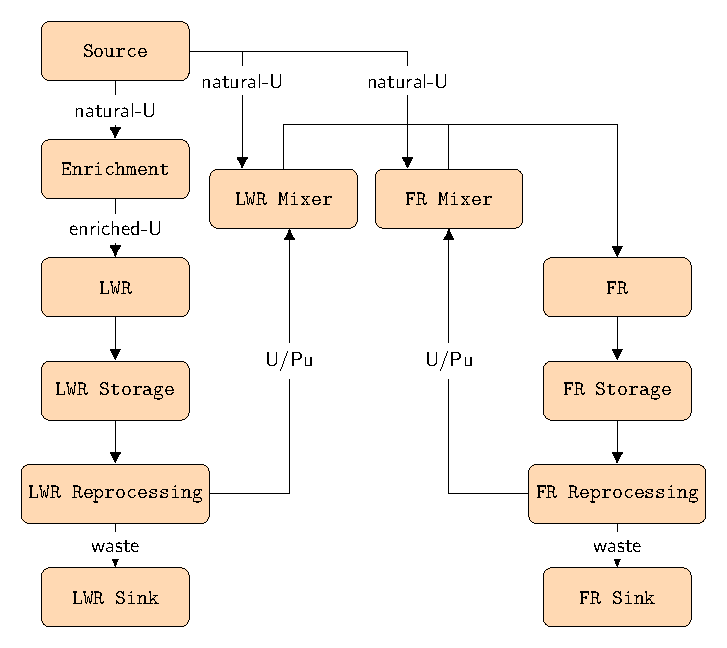
\includegraphics[width=0.55\linewidth]{23flow.pdf} 
		\caption{EG01-EG23.}
		\label{fig:23flow}
	\end{subfigure}
	\vspace{1cm}
	\begin{subfigure}[t]{\textwidth}
		\centering
		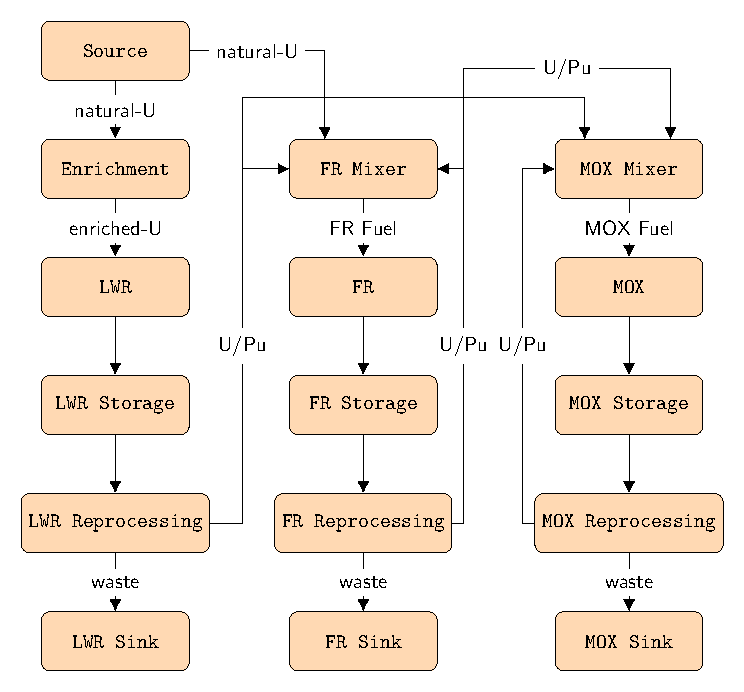
\includegraphics[width=0.55\linewidth]{29flow.pdf} 
		\caption{EG01-EG29.}
		\label{fig:29flow}
	\end{subfigure}
	\hfill
	\caption{Diagrams with facilities and mass flow of the scenarios EG01-EG23 and EG01-EG29.}
	\label{fig:eg2329}
\end{figure}

In Figure \ref{fig:eg23under}, crosses represent the time steps in which there is 
undersupply or under capacity of each commodity for a constant power 
EG01-23 scenario for varying prediction methods.
The size of the crosses are proportional to the undersupply
value, therefore, larger crosses correspond to larger undersupply. 
Table \ref{tab:all-power} shows the number of time steps with power 
undersupply for constant power EG01-EG23 and EG01-29, 
linearly increasing power EG01-24 and EG01-30 transition scenarios. 
Figure \ref{fig:eg23under} demonstrates that the \texttt{poly} and 
\texttt{fft} methods perform the best, since they have the least number 
of points on the plot, indicating that they have the fewest number of time 
steps with undersupply and under capacity of commodities. 
Table \ref{tab:all-power} shows that the \texttt{poly} method performs slightly 
better at minimizing undersupply of power than \texttt{fft}.
A similar analysis was done for a constant power EG01-29 scenario, and as seen 
in Table \ref{tab:all-power}
the \texttt{poly} prediction method also performed best for minimizing undersupply 
of power.  

In Figure \ref{fig:eg24under}, crosses represent the time steps in which there is undersupply 
or under capacity of each commodity for a linearly increasing power EG01-24 
scenario for varying prediction methods.
As with Figure \ref{fig:eg23under}, the size of the crosses are 
proportional to the undersupply value. 
Figure \ref{fig:eg24under} demonstrates that the \texttt{fft} method 
performs the best at minimizing undersupply of all commodities.
A similar analysis was performed for a constant power EG01-30 scenario, and 
as seen in Table \ref{tab:all-power} the \texttt{fft} also performed 
best for minimizing undersupply of power. 

\begin{figure}[]
	\centering
	\begin{subfigure}[t]{1.2\textwidth}
		\centering
		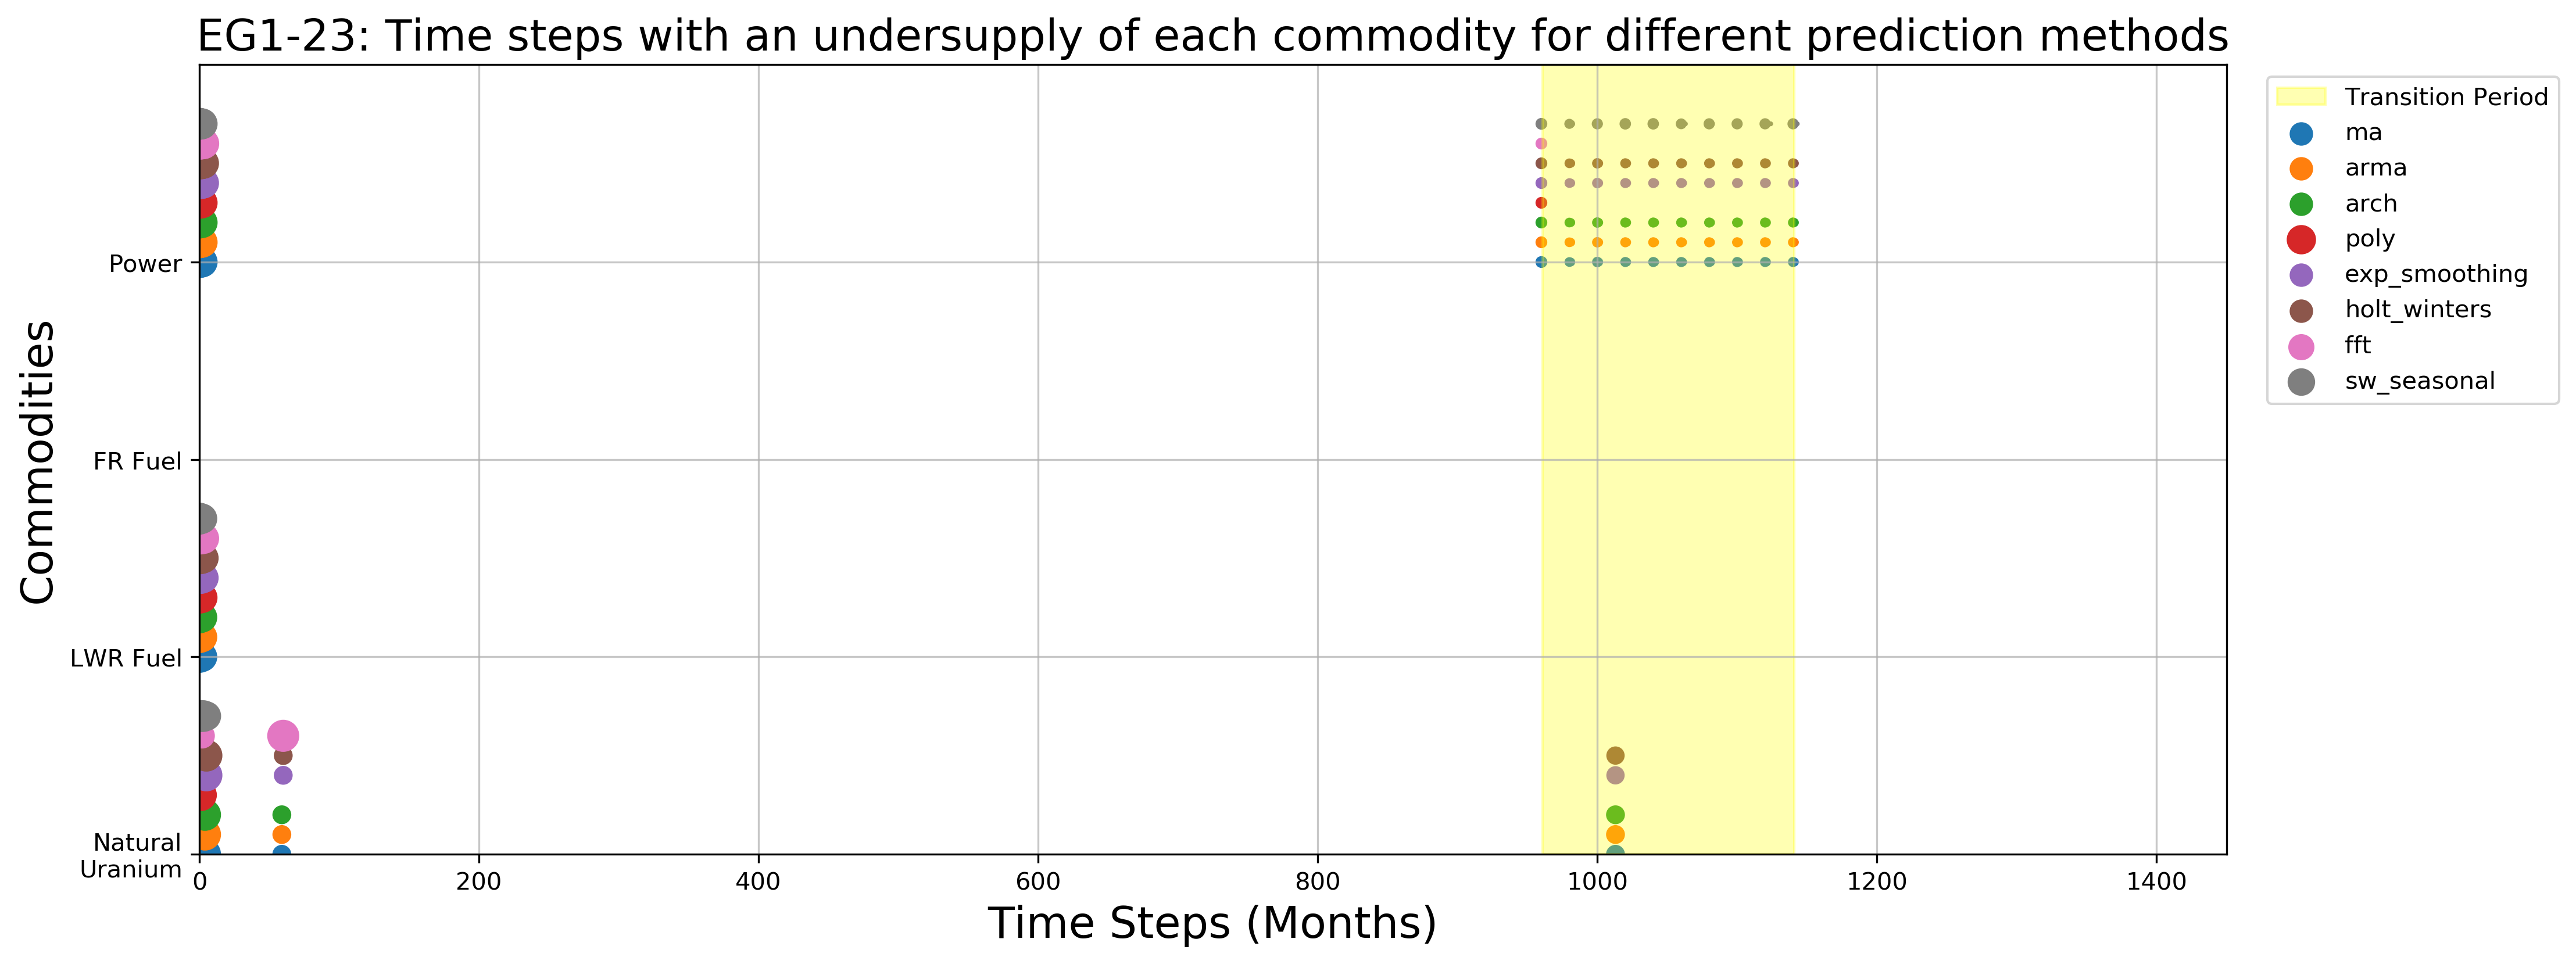
\includegraphics[width=\linewidth]{eg23-undersupply.png} 
		\caption{Time dependent undersupply of commodities in simulation }
		\label{fig:23undersupply}
	\end{subfigure}
	\vspace{1cm}
	\begin{subfigure}[t]{1.2\textwidth}
		\centering
		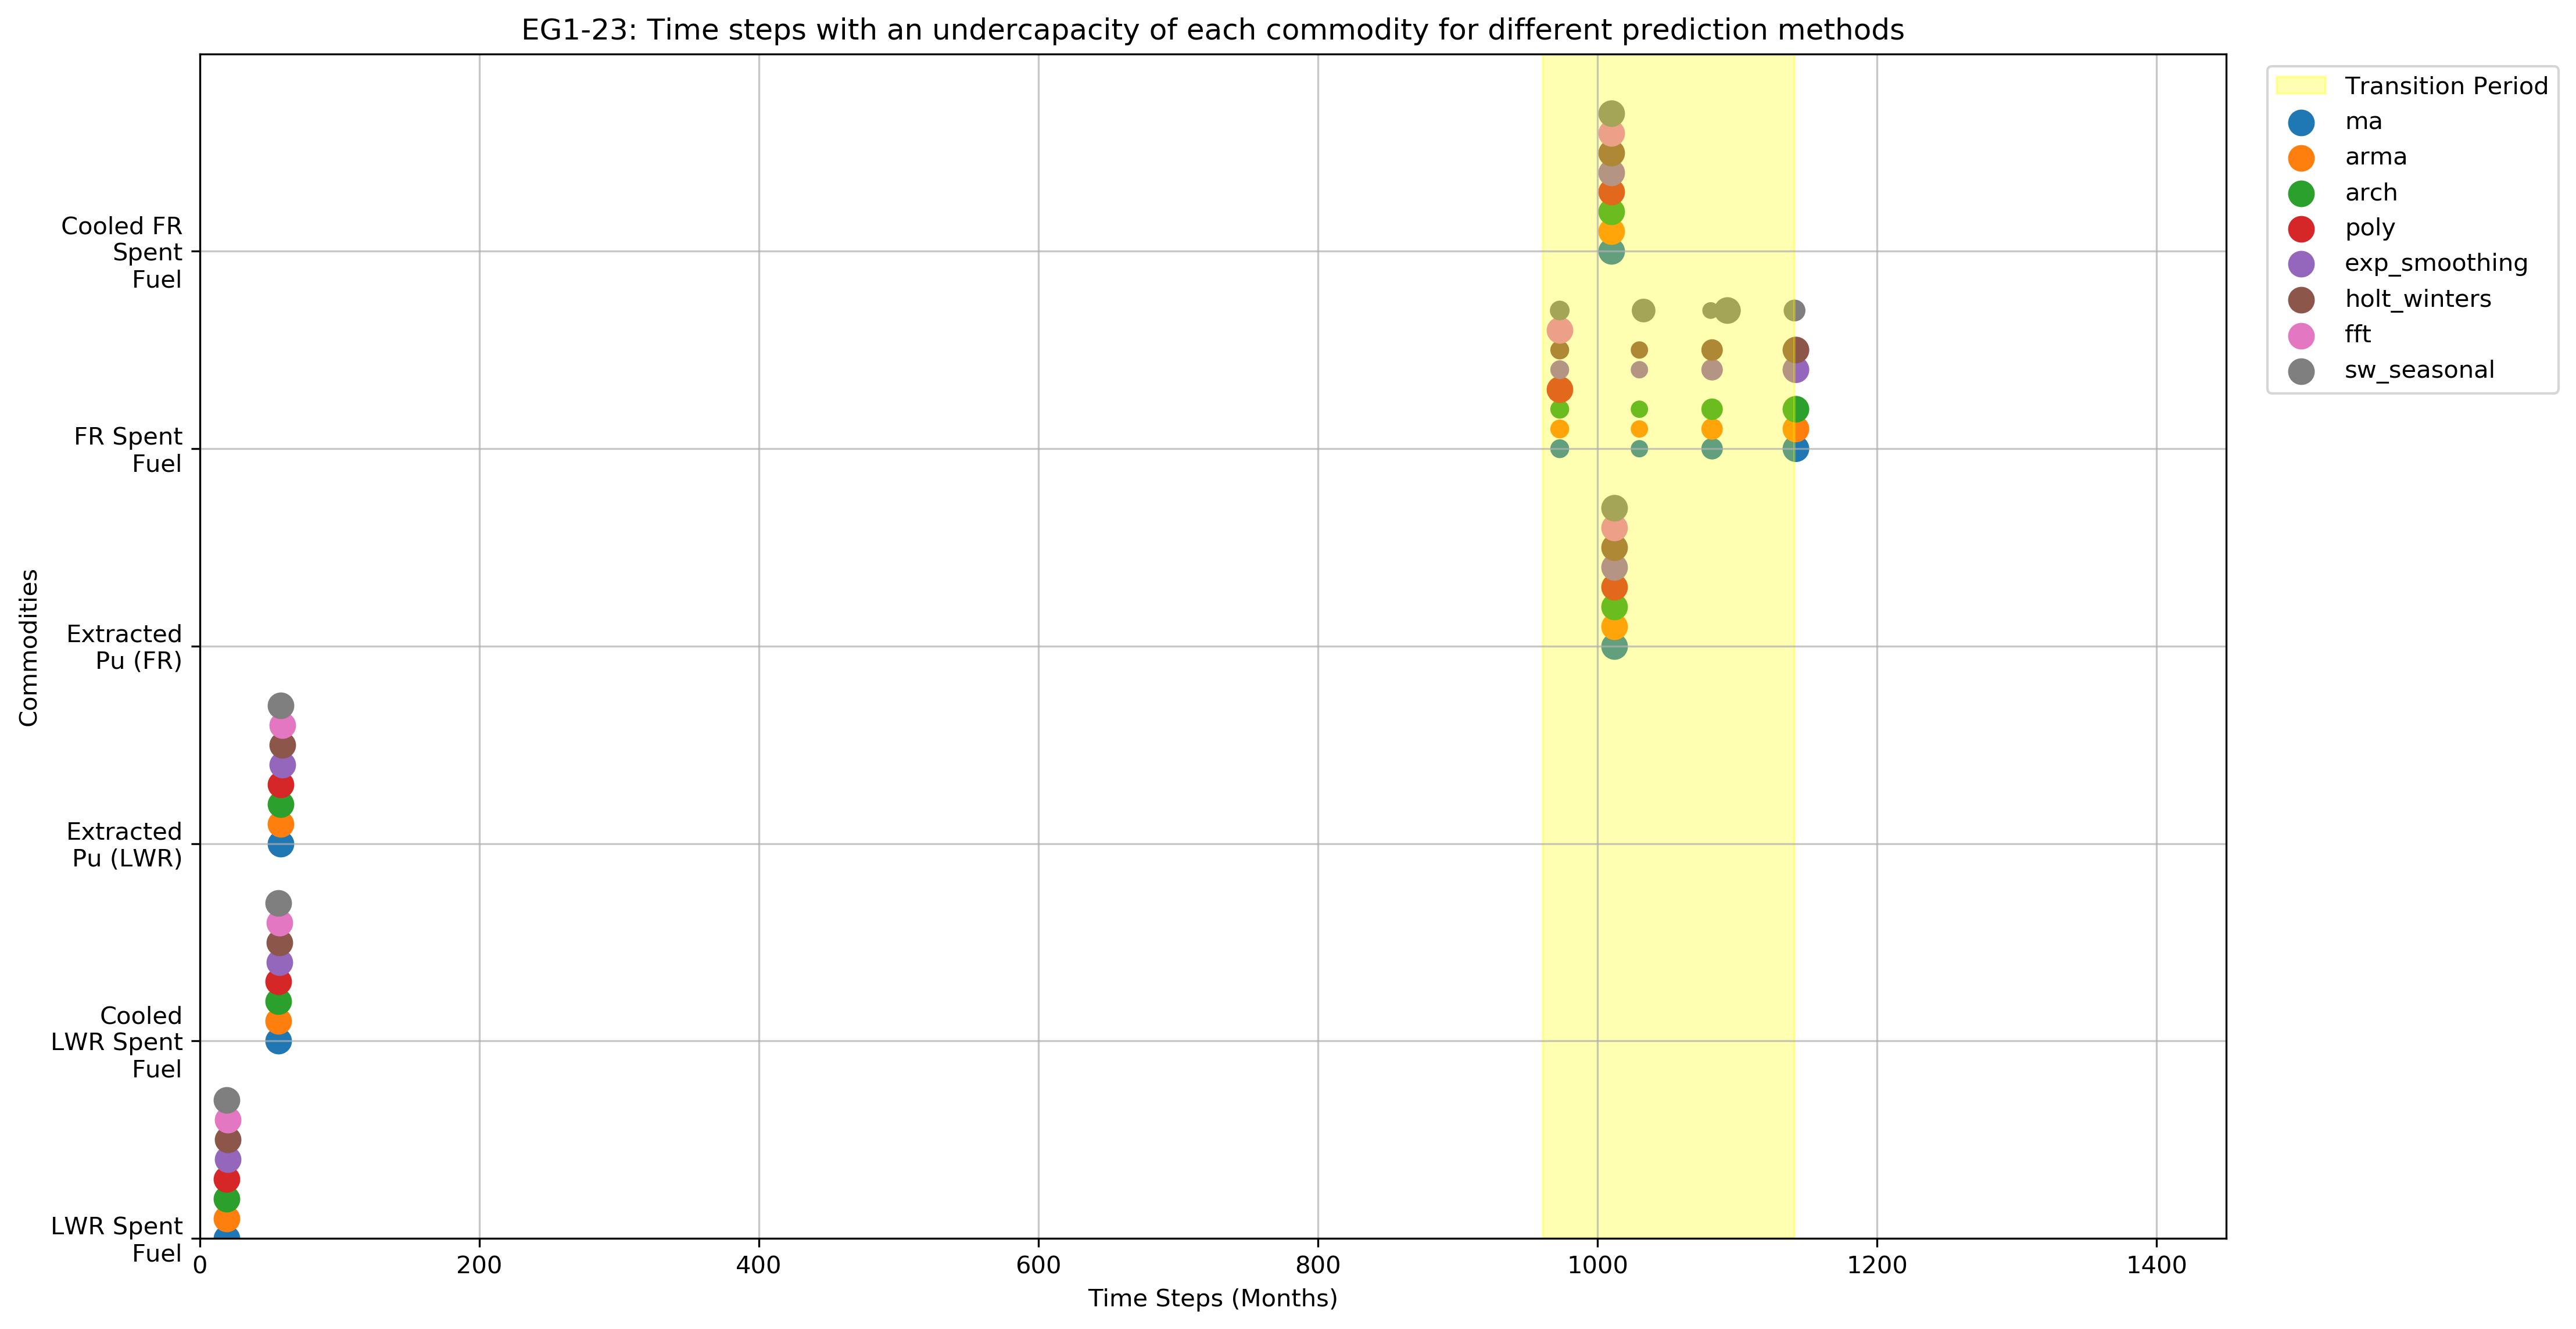
\includegraphics[width=\linewidth]{eg23-undercapacity.png} 
		\caption{Time dependent under capacity of commodities in simulation }
		\label{fig:23undercapacity}
	\end{subfigure}
	\hfill
	\caption{
	EG01-23 Transition Scenario with Constant Power Demand: 
	Each cross represent a time step in which there is undersupply 
	or under capacity of each commodity for varying prediction methods. 
	The size of each cross is proportional on the size of the undersupply.}
	\label{fig:eg23under}
\end{figure}

\begin{figure}[]
	\centering
	\begin{subfigure}[t]{1.2\textwidth}
		\centering
		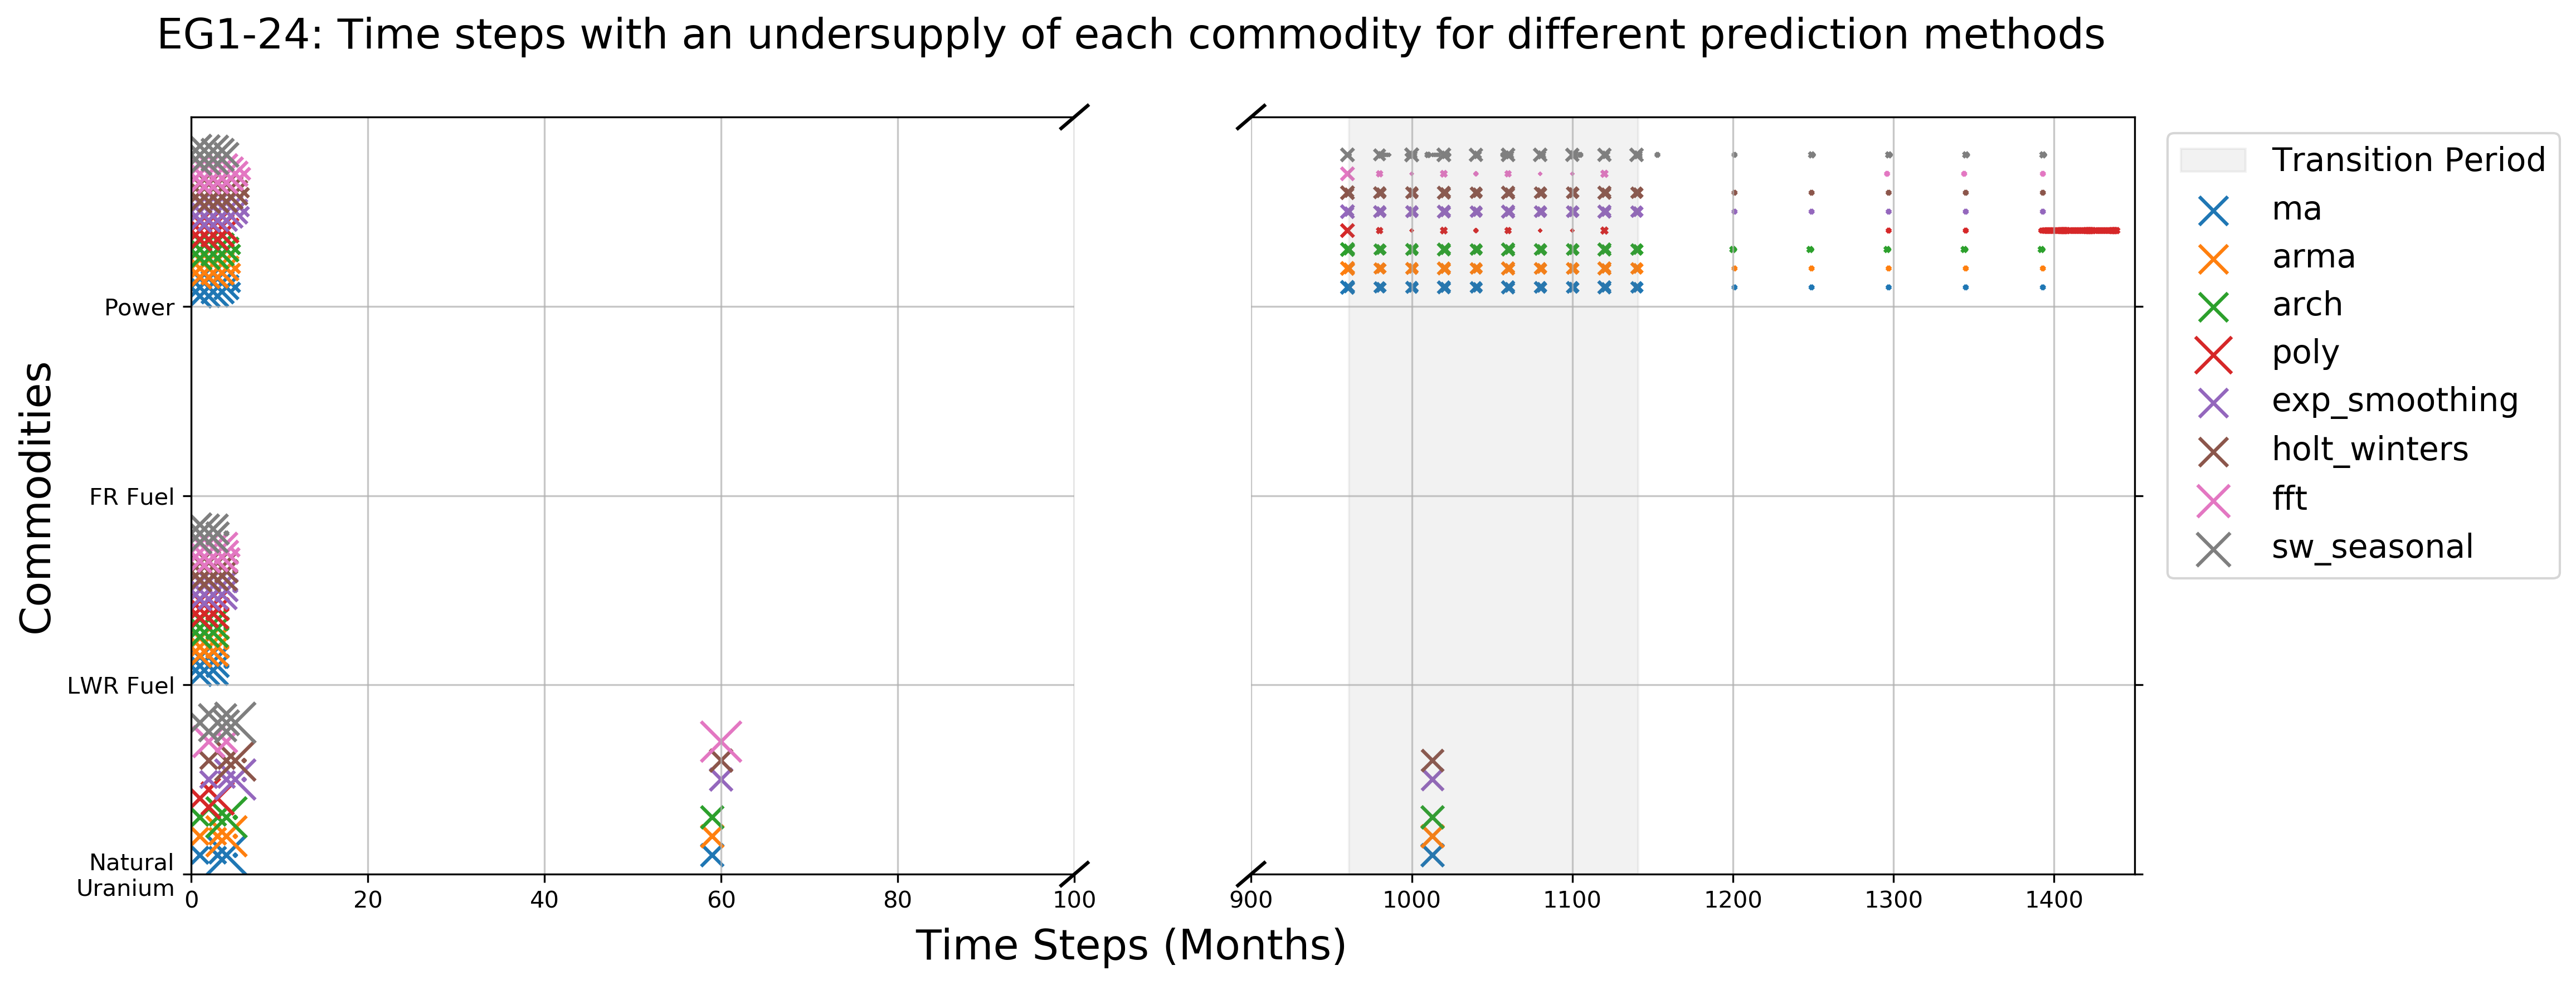
\includegraphics[width=\linewidth]{eg24-undersupply.png} 
		\caption{Time dependent undersupply of commodities in simulation }
		\label{fig:24undersupply}
	\end{subfigure}
	\vspace{1cm}
	\begin{subfigure}[t]{1.2\textwidth}
		\centering
		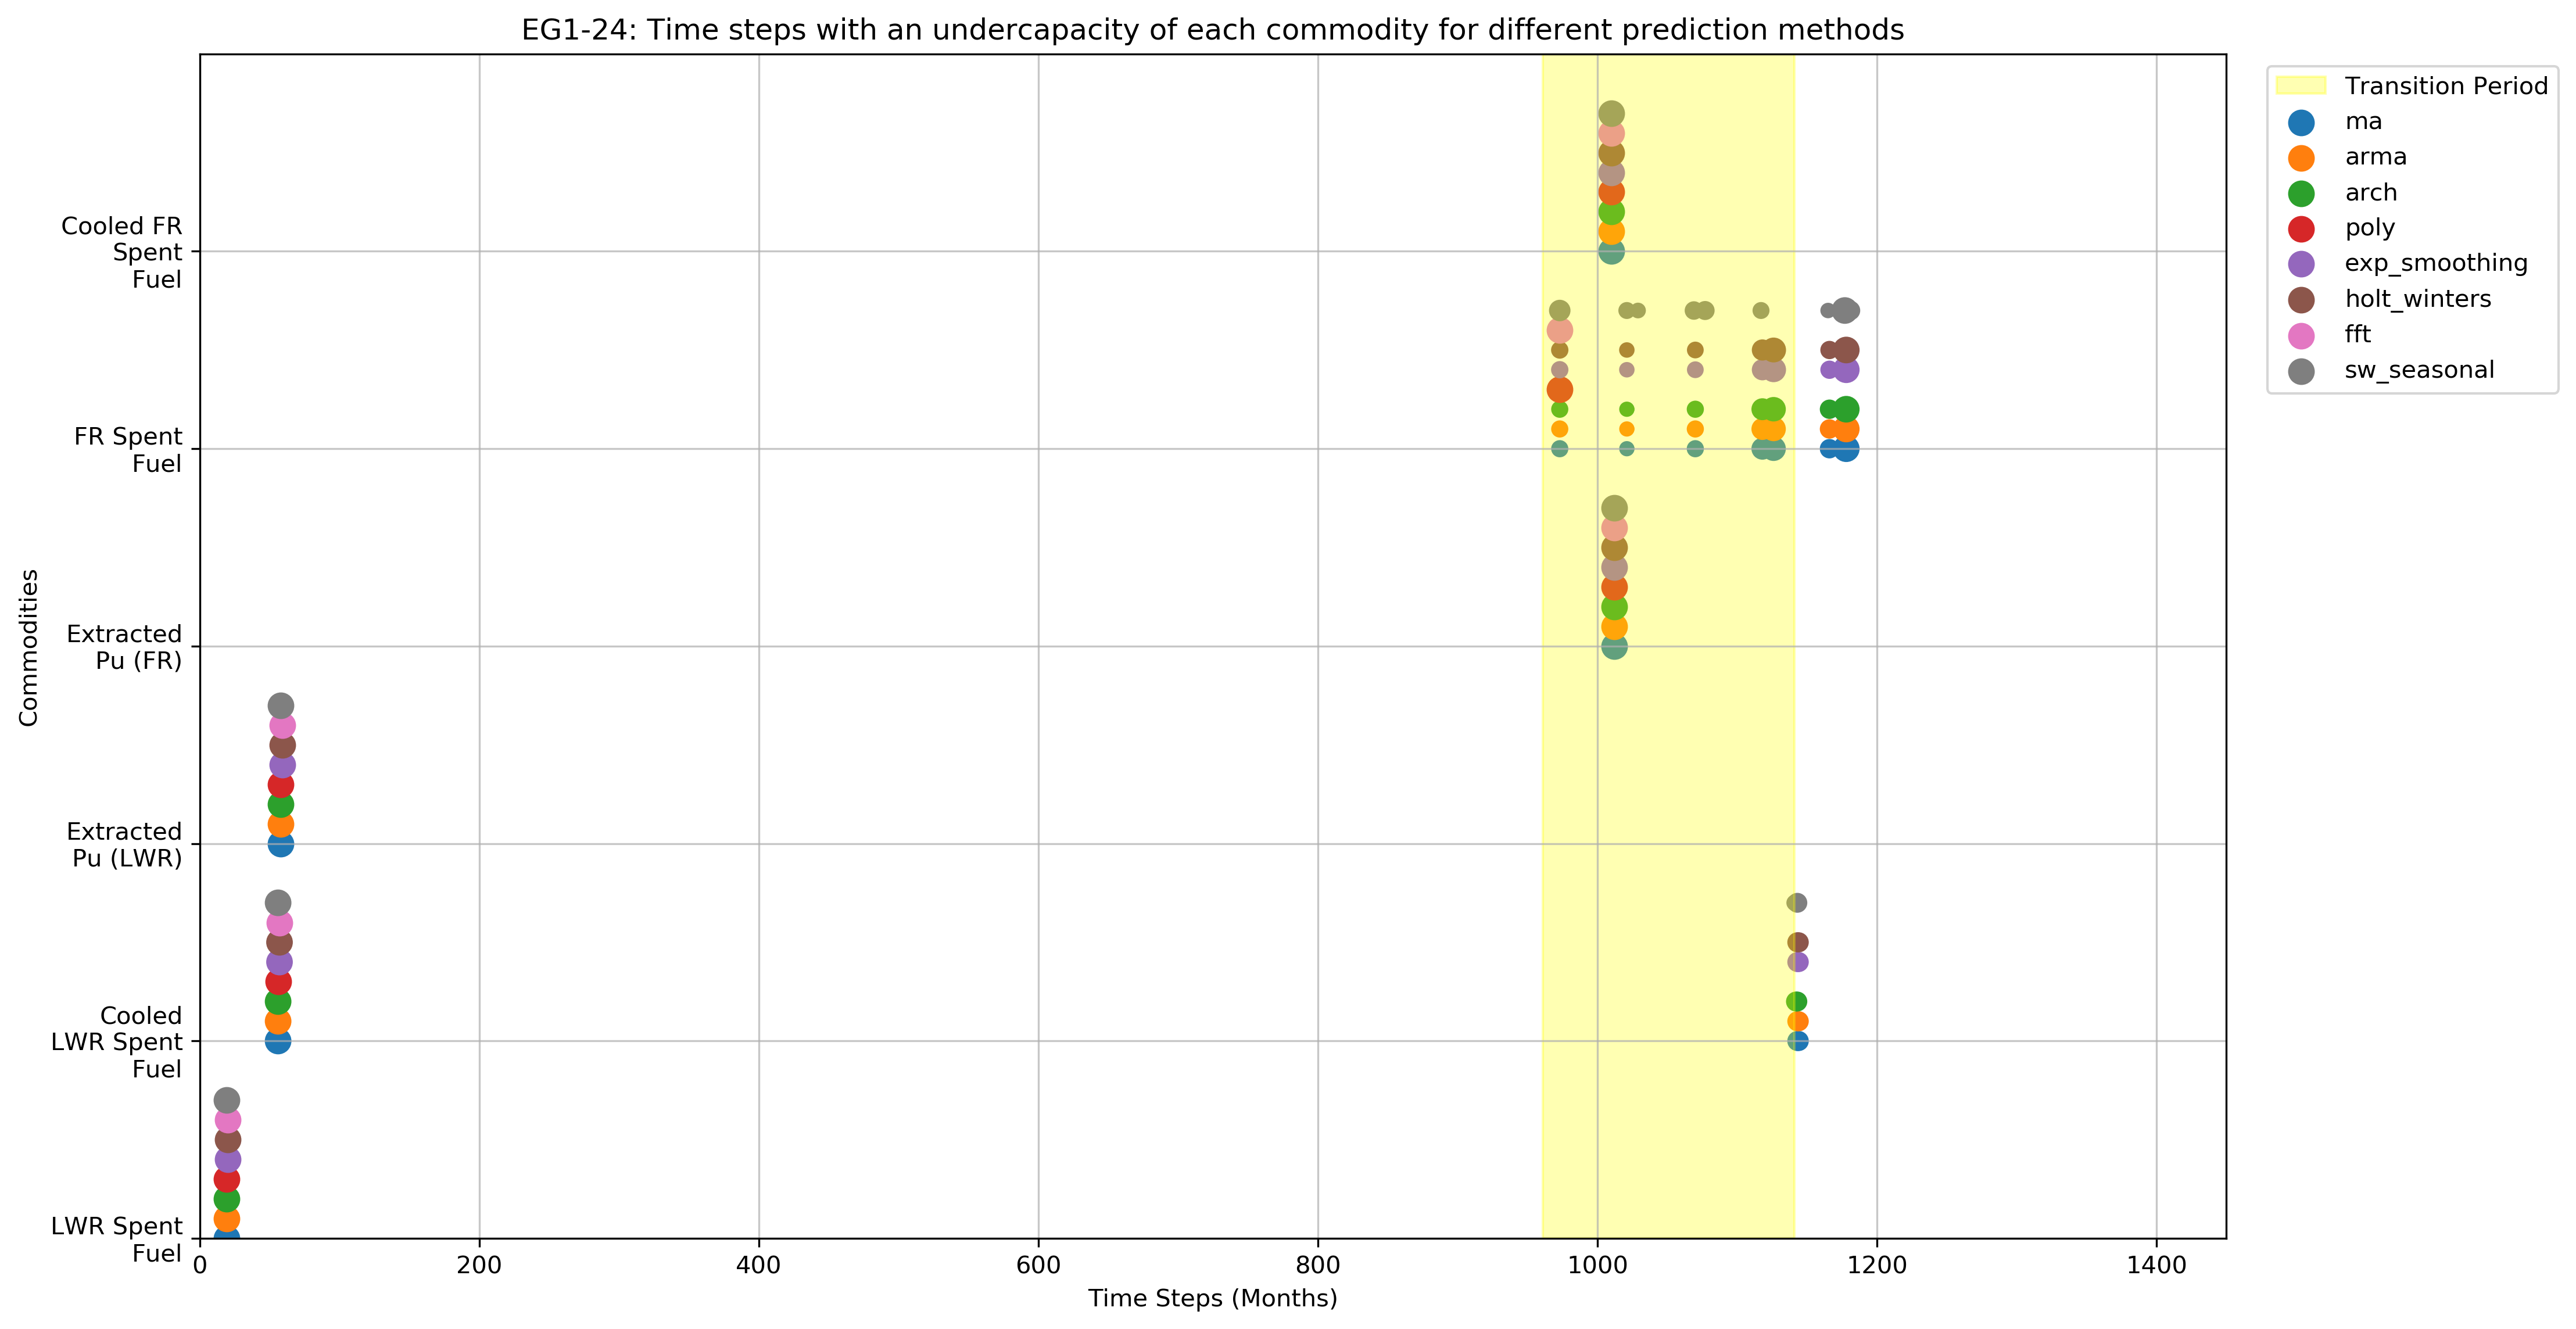
\includegraphics[width=\linewidth]{eg24-undercapacity.png} 
		\caption{Time dependent under capacity of commodities in simulation }
		\label{fig:24undercapacity}
	\end{subfigure}
	\hfill
	\caption{
	EG01-24 Transition Scenario with Linearly Increasing Power Demand:
	Each cross represent a time step in which there is undersupply 
	or under capacity of each commodity for varying prediction methods. 
	The size of each cross is proportional on the size of the undersupply.}
	\label{fig:eg24under}
\end{figure}

\begin{table}[]
	\centering
        \caption{Undersupply and oversupply of power with the different 
        algorithms used to drive EG01-EG23,24,29,30.}
		\label{tab:all-power}
		\footnotesize
        \begin{tabularx}{\textwidth}{l|RRRR}
		\hline
		& \multicolumn{3}{|c}{\textbf{Power Undersupplied Time Steps}} \\ \hline
		Algorithm & EG01-EG23 Constant Power  & 
		EG01-EG24 Linearly Increasing Power   & EG01-EG29 Constant Power & 
		EG01-EG30 Linearly Increasing Power \\ \hline
		MA     		    & 26 	& 36  &  15  & 24 \\ 
		ARMA     	    & 26 	& 36  &  15  & 24\\ 
		ARCH     	    &  26 	& 36  &  15  & 21\\ 
		POLY      		&  6 	& 65  &  4 &  9\\ 
		EXP\_SMOOTHING 	& 27 	& 37  & 16 & 25\\ 
		HOLT-WINTERS  	& 27 	& 37  & 16 & 25\\ 
		FFT       		& 8 	& 20  & 5 & 9\\ 
		SW\_SEASONAL    & 36 	& 107 & 14 & 51\\ \hline
	\end{tabularx}
\end{table}

From Figures \ref{fig:eg23under}, \ref{fig:eg24under}, and Table 
\ref{tab:all-power}, we can see that the \texttt{poly} method 
performs best for constant power transition scenarios
and the \texttt{fft} method performs best for linearly increasing 
power transition scenarios. 
Undersupply and under capacity of commodities occur during two main time periods: 
initial demand for the commodity and during the transition period.
To further \deploy's main objective of minimizing the power undersupply, 
sensitivity analysis of the power supply 
buffer for each transition scenario is conducted 
with best performing prediction method
to find a buffer size that will minimize power 
undersupply.  

\subsection{Sensitivity Analysis}
Sensitivity analysis of the power buffer size was conducted for 
EG01-EG23, EG01-24, EG01-29, and EG01-30 transition scenarios. 
Varying the power buffer size does not impact the number of 
undersupply time steps for EG01-EG23 and EG01-EG29 constant 
power demand transition scenario with the \texttt{poly} prediction method.
There are 6 and 4 time steps (table \ref{tab:all-power}) 
in which there is power undersupply for EG01-EG23 and EG01-29 
transition scenarios respectively. 
As seen from figure \ref{fig:eg23under}, these undersupply time 
steps occur at the beginning of the simulation and for one 
time step when the transition begins. 
This is expected since without time series data 
at the beginning of the simulation, \deploy takes a few 
time steps to collect time series data about power demand 
to predict and start deploying reactor and supporting 
fuel cycle facilities. 
When the transition begins, power is under supplied for one 
time step, ; following this, \deploy accounts for the 
undersupply by deploying facilities to meet power demand.
Therefore, the power undersupply is minimized for constant 
power EG01-EG23 and EG01-EG29 transition scenarios with 
a 0MW power supply buffer. 

For EG01-EG24 and EG01-30 linearly increasing power demand 
transition scenarios, power buffer size is varied.  
Figures \ref{fig:eg24-bufplot}, \ref{fig:eg30-bufplot} 
and Table \ref{tab:buff_size} 
show that with an increasing buffer size, the number of 
power undersupply time steps decreases. 
For EG01-24, it plateaus at 6000MW, and for EG01-30, 
the cumulative undersupply is smallest for a buffer 
size of 8000MW.  
As seen from Figures \ref{fig:eg24-dotplot} and 
\ref{fig:eg30-dotplot}, these undersupply time 
steps occur at the beginning of the simulation and for one 
time step when the transition begins. 
This is expected since without time series data 
at the beginning of the simulation, \deploy takes a few 
time steps to collect time series data about power demand 
to predict and start deploying reactor and supporting 
fuel cycle facilities. 
Therefore, a buffer of 6000MW and 8000MW minimizes 
the power undersupply for EG01-Eg24 and EG01-EG30 respectively.

\begin{figure}[]
	\centering
	\begin{subfigure}[t]{0.8\textwidth}
		\centering
		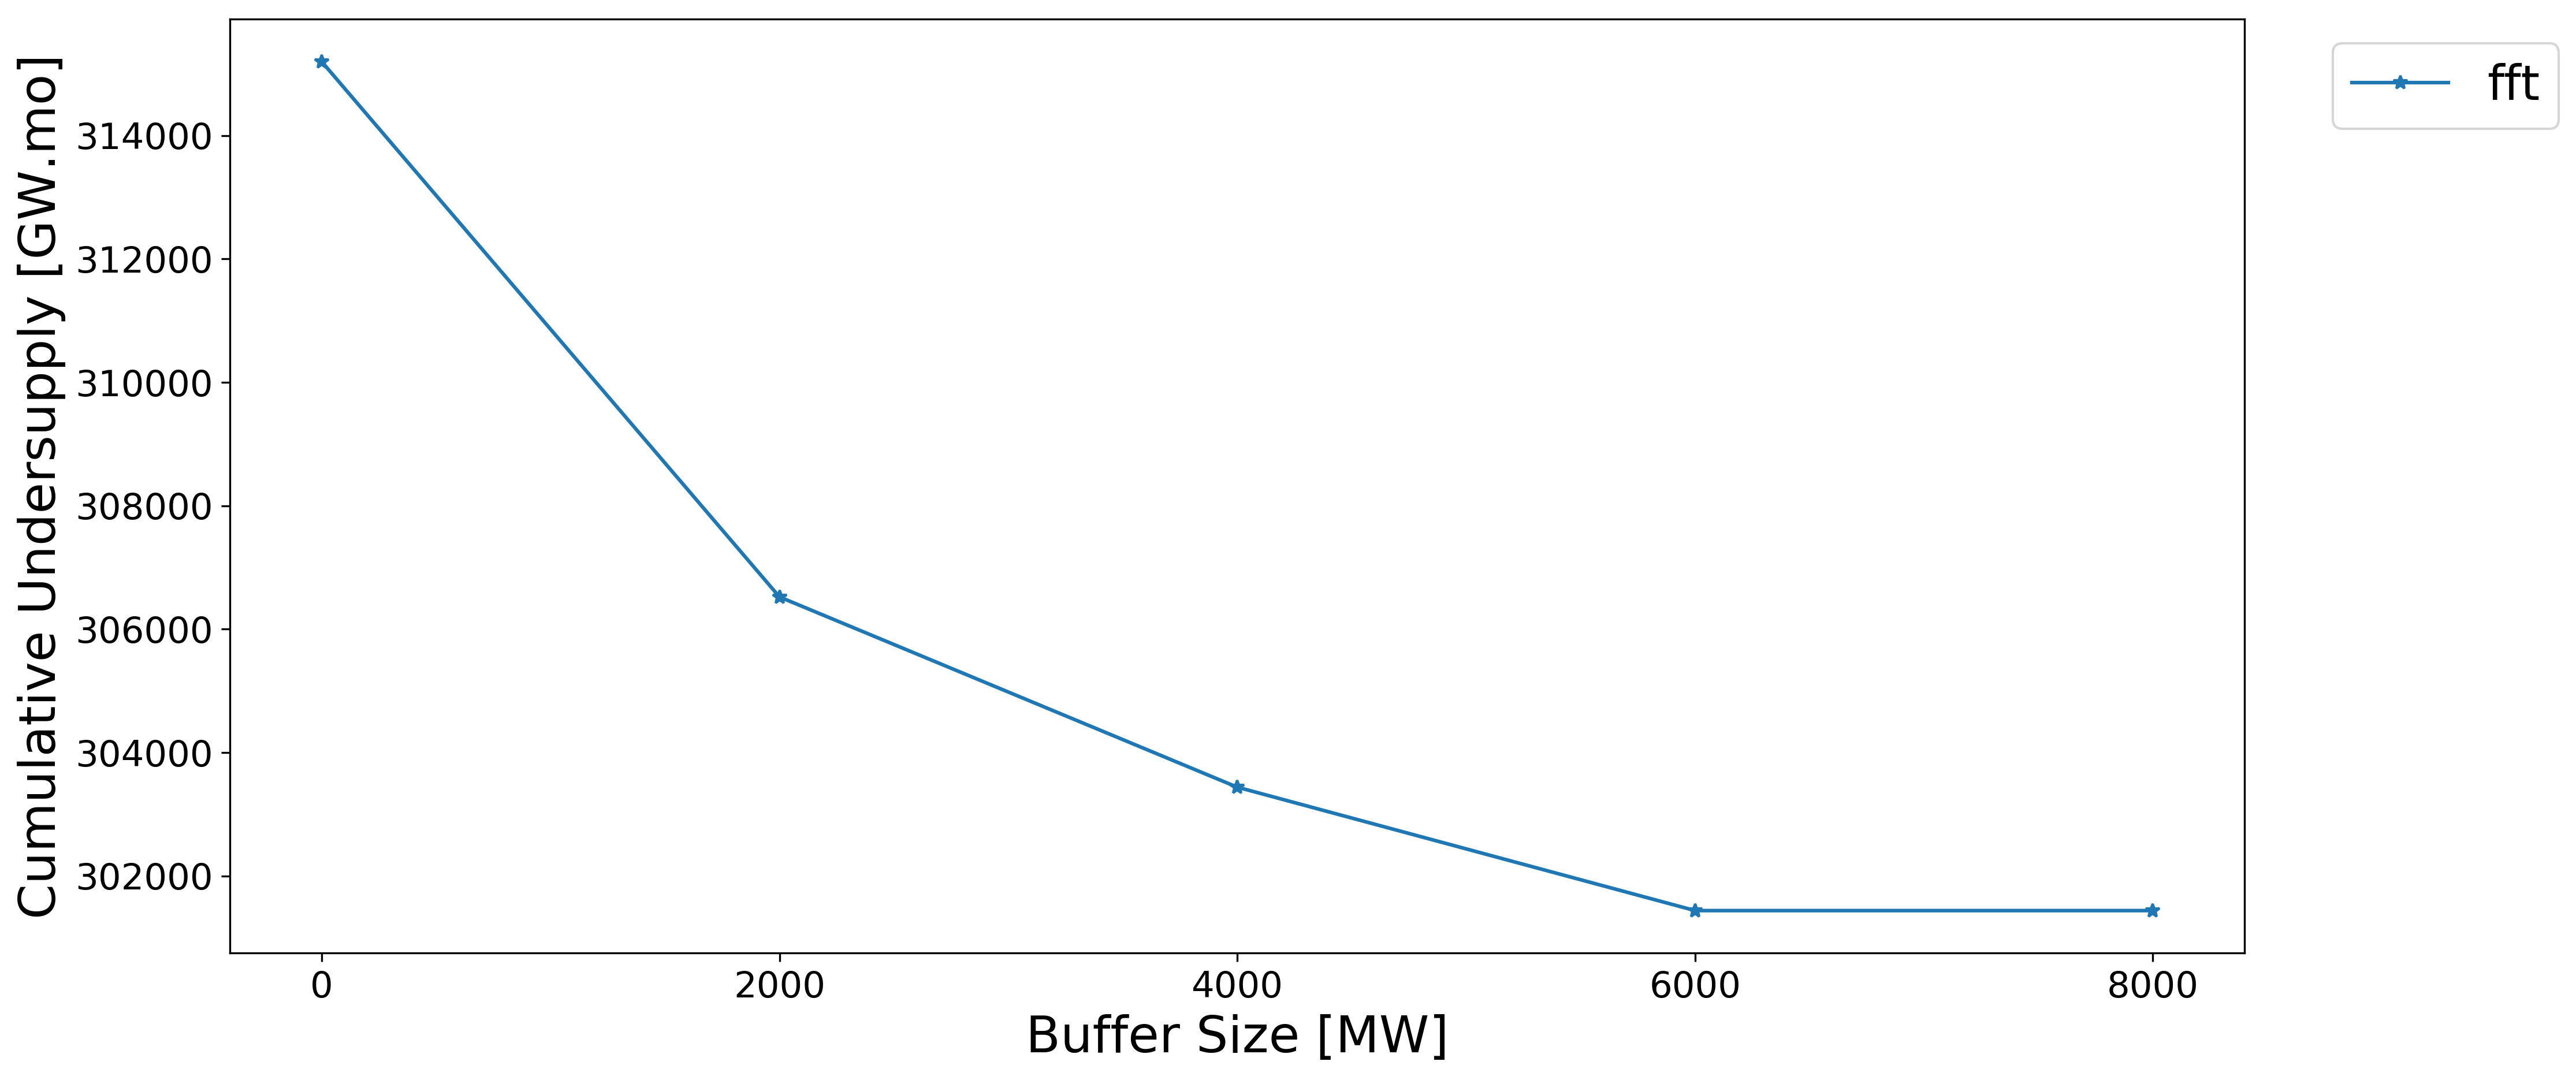
\includegraphics[width=\linewidth]{24-sens-buffer.png} 
		\caption{EG01-24: Power buffer size vs. cumulative undersupply}
		\label{fig:eg24-bufplot}
	\end{subfigure}
	\vspace{1cm}
	\begin{subfigure}[t]{0.8\textwidth}
		\centering
		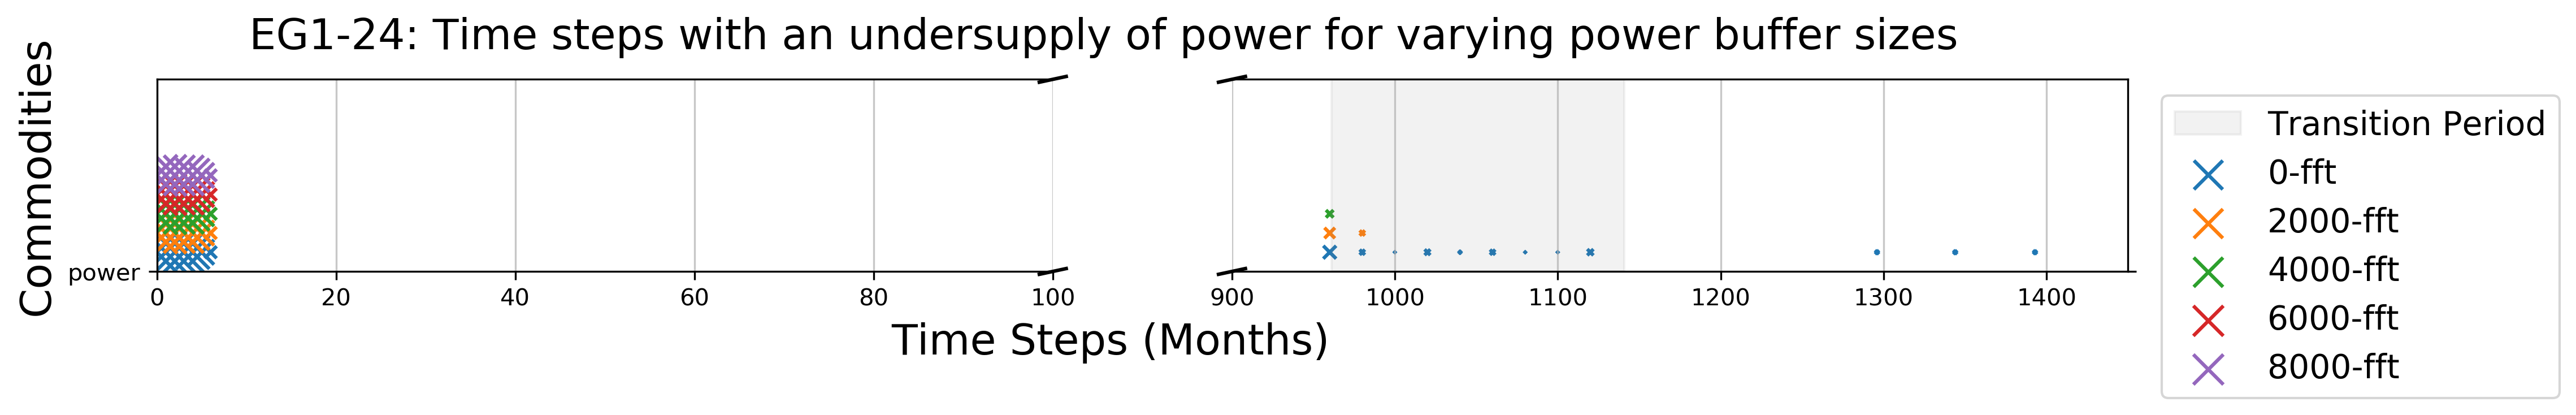
\includegraphics[width=\linewidth]{eg24-sa.png} 
		\caption{EG01-24: Time-dependent undersupply of power for varying power buffer sizes}
		\label{fig:eg24-dotplot}
	\end{subfigure}
	\begin{subfigure}[t]{0.8\textwidth}
		\centering
		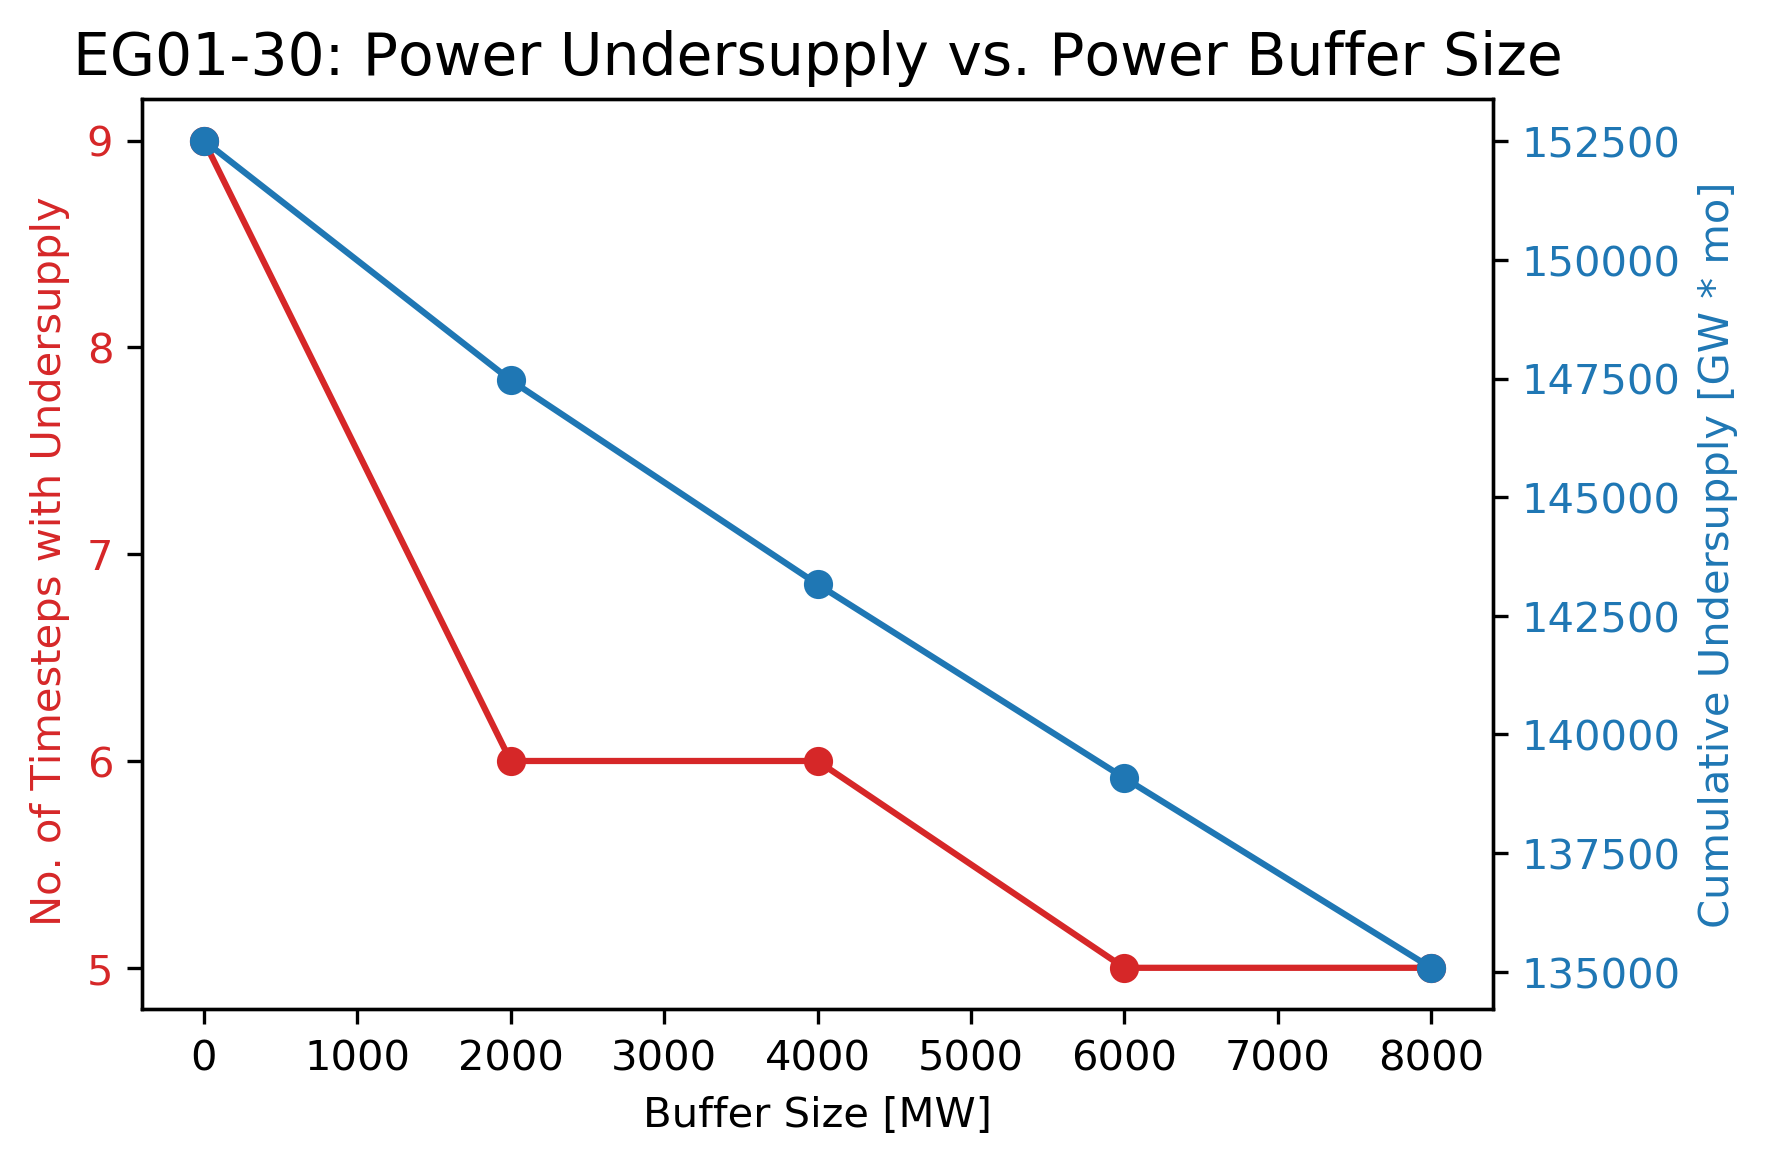
\includegraphics[width=\linewidth]{30-sens-buffer.png} 
		\caption{EG01-30: Power buffer size vs. cumulative undersupply}
		\label{fig:eg30-bufplot}
	\end{subfigure}
	\begin{subfigure}[t]{0.8\textwidth}
		\centering
		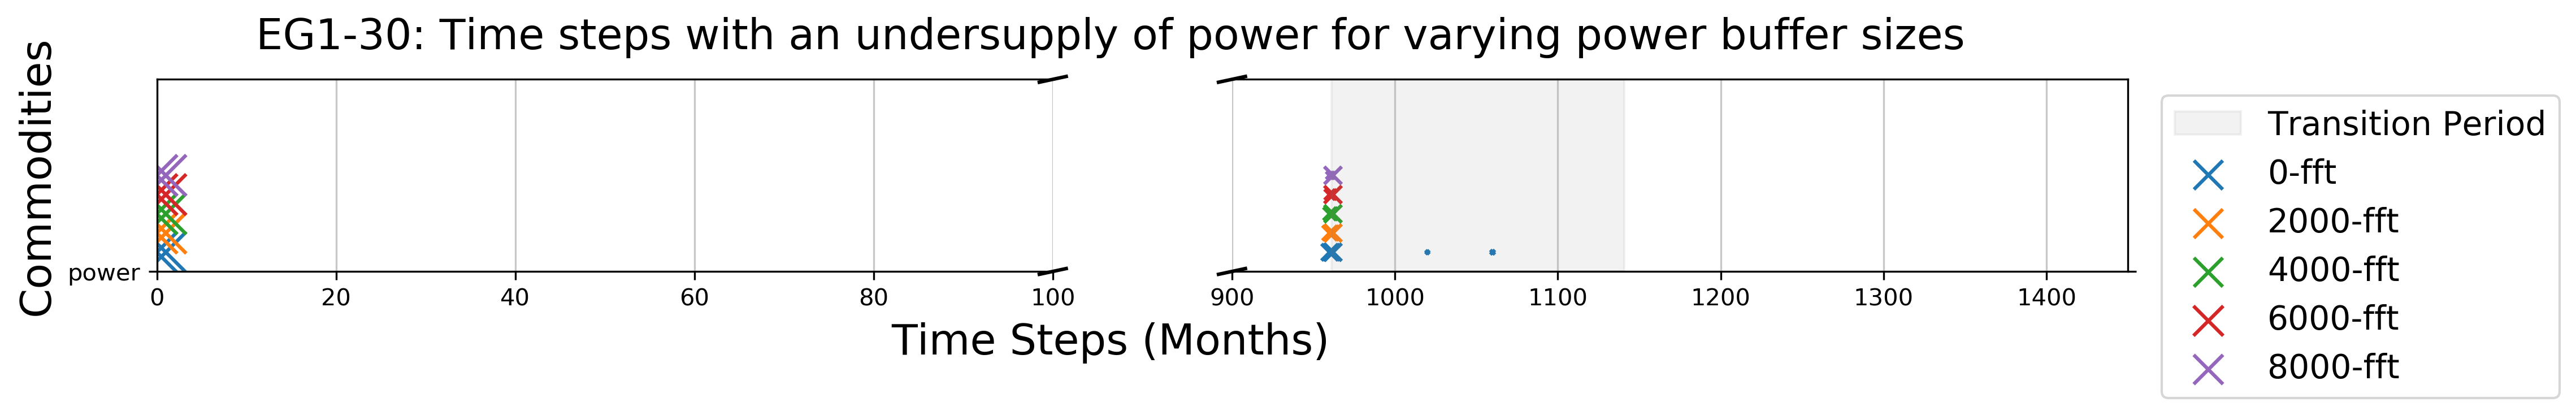
\includegraphics[width=\linewidth]{eg30-sa.png} 
		\caption{EG01-30: Time-dependent undersupply of power for varying power buffer sizes}
		\label{fig:eg30-dotplot}
	\end{subfigure}
	\hfill
	\caption{Sensitivity Analysis of Power buffer size on cumulative 
	undersupply of Power for EG01-EG24 and EG01-EG30 transition scenarios 
	with linearly increasing power demand using the fft prediction method.}
	\label{fig:sabuffer}
\end{figure}

\begin{table}[h]
	\centering
	\caption{Dependency of the undersupply of Power on the buffer size 
	for EG01-EG24 and EG01-EG30 transition scenarios with linearly 
	increasing power demand using the fft prediction method.}
	\label{tab:buff_size}
	\footnotesize
		\begin{tabularx}{\textwidth}{LLRR}
                \hline
        Buffer [MW]     & Undersupply             & EG01-24   & EG01-30 \\
		\hline
		0             & Time steps $[\#]$ & 20 & 9\\  
                      & Energy $[GW\cdot mo]$    & 315791 & 152517 \\ \hline
        2000          & Undersupplied $[\#]$ & 9 & 6 \\  
        	      & Energy $[GW\cdot mo]$    & 306520 & 147166 \\ \hline
        4000          & Time steps $[\#]$ & 8 & 6 \\  
				  & Energy $[GW\cdot mo]$    & 303438 & 143166 \\ \hline
		6000          & Time steps $[\#]$ & 7 & 5 \\  
		& Cumulative $[GW]$    & 303438 & 139083 \\ \hline
        8000          & Time steps $[\#]$ & 7 & 5  \\  
	              & Energy $[GW\cdot mo]$    & 303438 & 135083 \\ \hline
	\end{tabularx}
\end{table}

\subsection{Best Performance Models}
Table \ref{tab:bestinputs} 
shows \deploy input parameters for
EG01-EG23, EG01-EG24, EG01-EG29, and EG01-EG30 transition scenarios
that minimize undersupply of power and minimize 
the undersupply and under capacity of the other commodities
in the simulation. 
The need for buffers for commodities is a reflection of reality
in which a supply buffer is usually maintained to ensure 
continuity in the event of an unexpected failure in the supply chain.

Figure \ref{fig:23stack} and \ref{fig:30stack} show
time dependent deployment of reactor and supporting facilities for 
the EG01-23 constant power demand and EG01-30 linearly increasing power demand 
transition scenarios, respectively. 
\deploy automatically deploys reactor and supporting facilities 
to setup a supply chain to meet power demand
during a transition from \glspl{LWR} to \glspl{SFR} for EG01-23, 
and from \glspl{LWR} to \gls{MOX} \glspl{LWR} and \glspl{SFR} for 
EG01-30. 
EG01-24 and EG01-29 facility deployment plots are very similar to 
EG01-23 and EG01-30, respectively, therefore they are not shown. 

\begin{table}[]
	\resizebox{\textwidth}{!}{%
	\begin{tabular}{l|l|c|l|l|l}
	\hline
	\multirow{2}{*}{}                         & \multicolumn{1}{c|}{\multirow{2}{*}{\textbf{Input Parameter}}} & \multicolumn{4}{c}{\textbf{Simulation Description}}                                                                                                                                                                                                                                                       \\ \cline{3-6} 
											  & \multicolumn{1}{c|}{}                                          & \multicolumn{1}{l|}{\textbf{EG01-23}}                                                                 & \textbf{EG01-24}                  & \textbf{EG01-29}                 &\textbf{EG01-30}                                                  \\ \hline
	\multirow{4}{*}{\textbf{Required}} & Demand driving commodity                                       & \multicolumn{4}{c}{Power}                                                                                                                                                                                                                                                                                 \\ \cline{2-6} 
											  & Demand equation [MW]                                               & \multicolumn{1}{l|}{60000}                                                                                & $60000 + 250t/12$ & 60000                     &     $60000 + 250t/12$                                       \\ \cline{2-6} 
											  & Prediction method                                              & \texttt{poly}       & \texttt{fft}             & \texttt{poly}         &  \texttt{fft}    \\ \cline{2-6} 
											  & Deployment Driving Method                                      & \multicolumn{4}{c}{Installed Capacity}                                                                                                                                                                                                                                                                    \\ \hline
	\multirow{2}{*}{\textbf{Optional}} & Buffer type                                                    & \multicolumn{4}{c}{Absolute}                                                                                                                                                                                                                                                               \\ \cline{2-6} 
											  & Power Buffer size [MW]                                                   & 0 & 6000 & 0 & 8000 \\ \hline
	\end{tabular}%
	}
	\caption{\deploy's input parameters for EG01-EG23, EG01-EG24, EG01-EG29, and 
	EG01-EG30 transition scenarios
	that minimizes undersupply of power and minimizes 
	the undersupply and under capacity of the other facilities. }
	\label{tab:bestinputs}
	\end{table}

\begin{figure}[]
	\centering
	\begin{subfigure}[t]{1.2\textwidth}
		\centering
		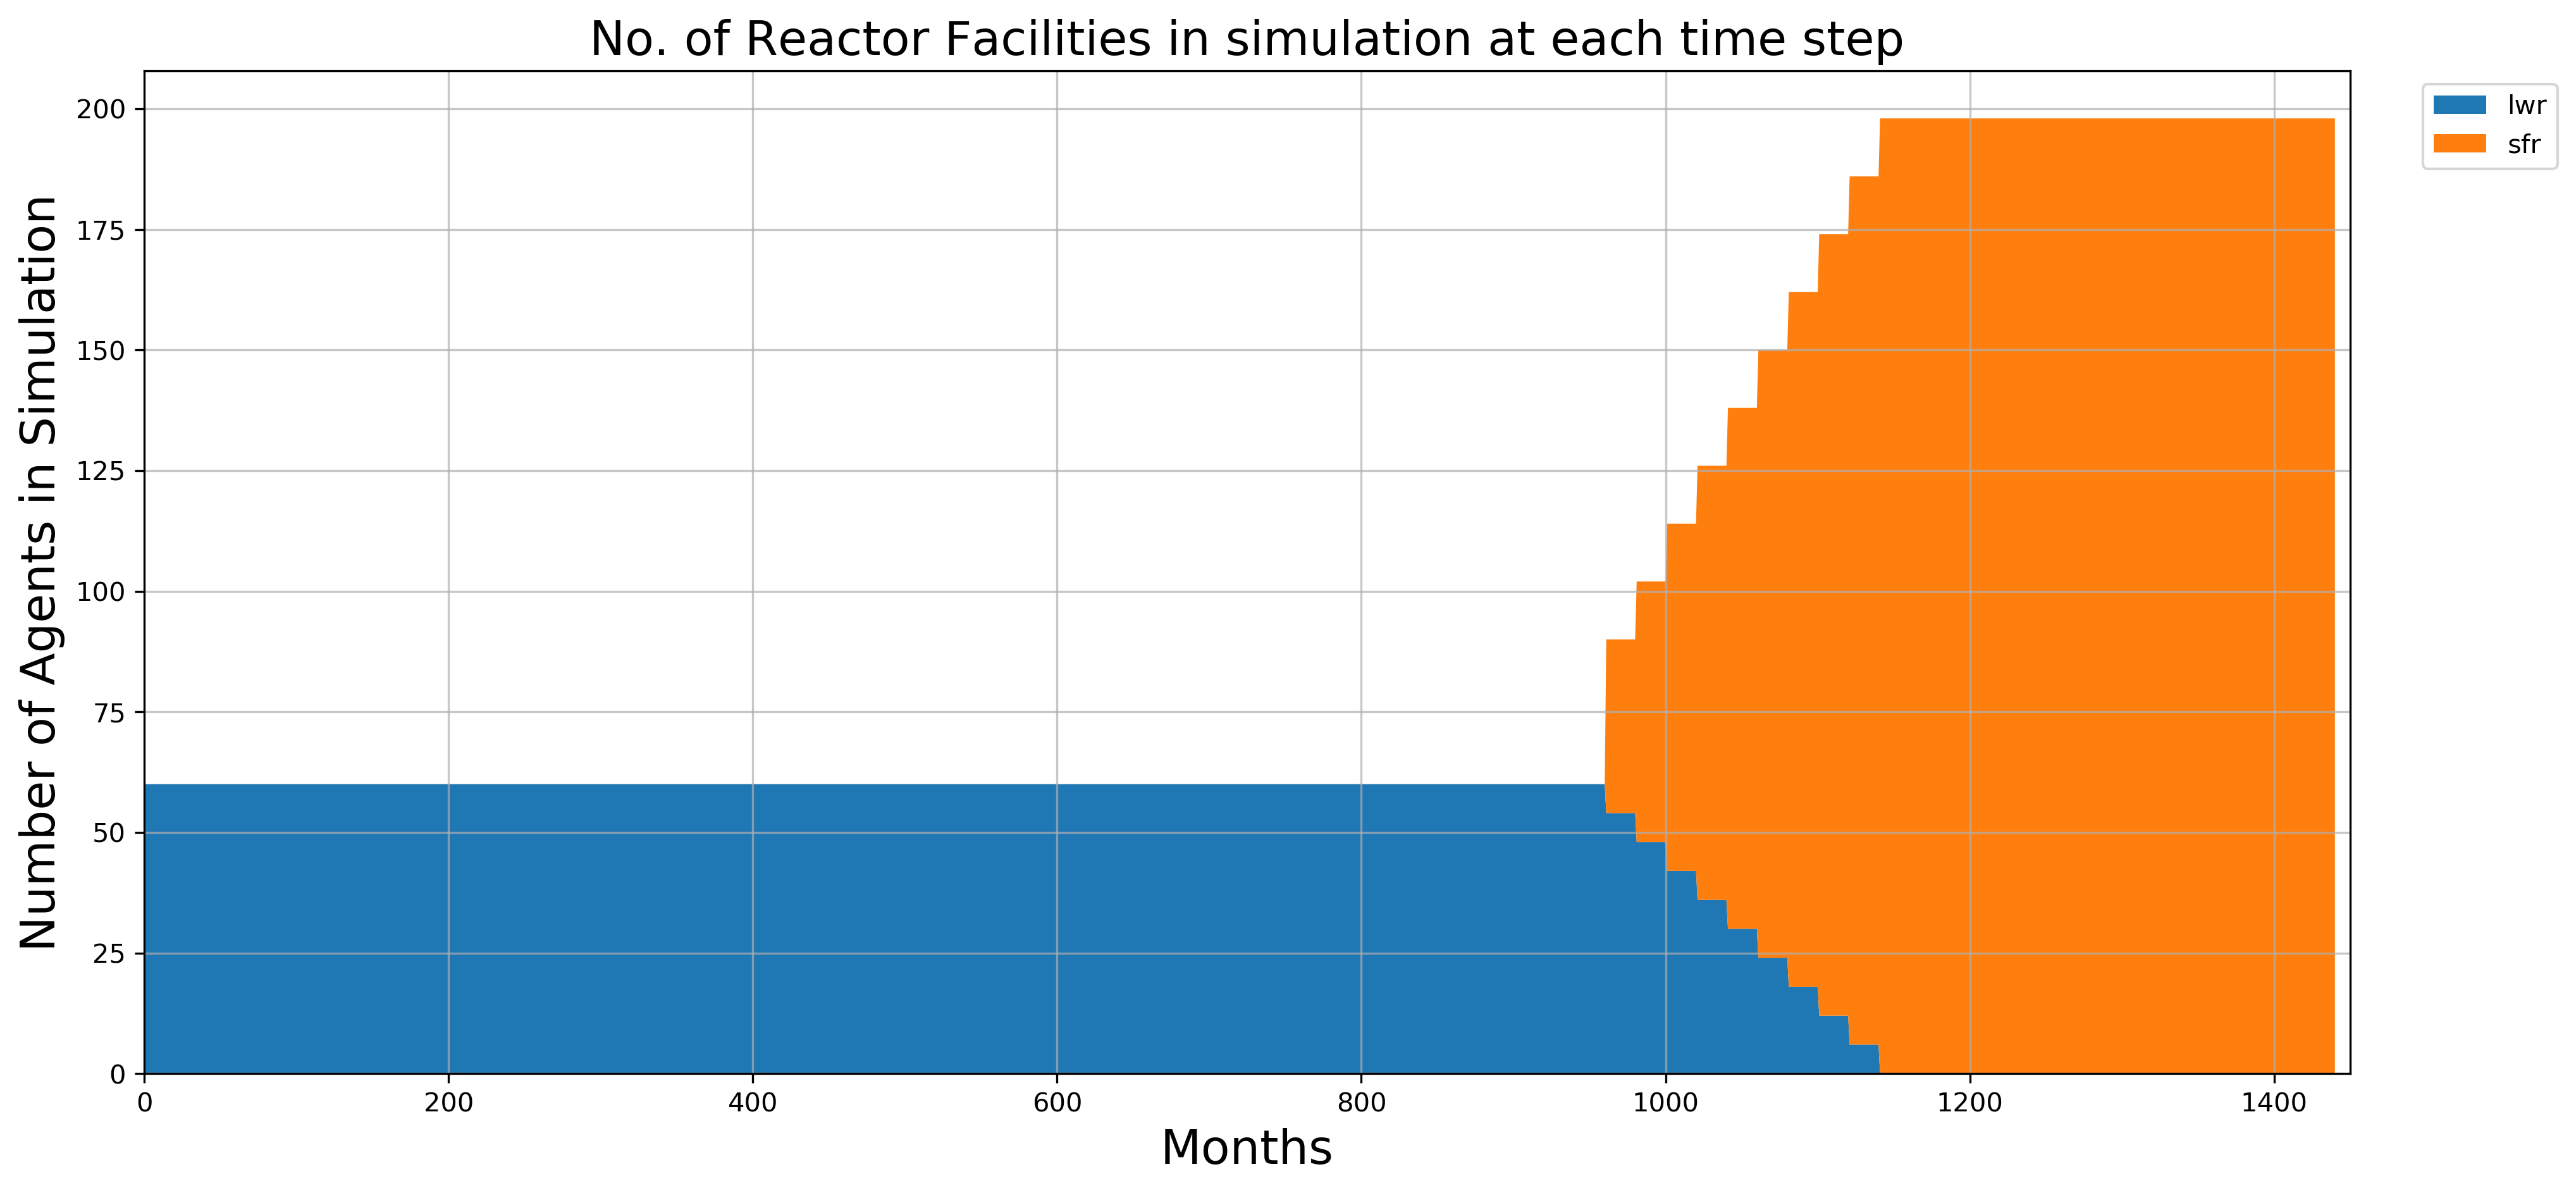
\includegraphics[width=\linewidth]{eg23-stack_reactor.png} 
		\caption{EG01-23: Reactor Deployment}
		\label{fig:23reactor}
	\end{subfigure}
	\vspace{1cm}
	\begin{subfigure}[t]{1.2\textwidth}
		\centering
		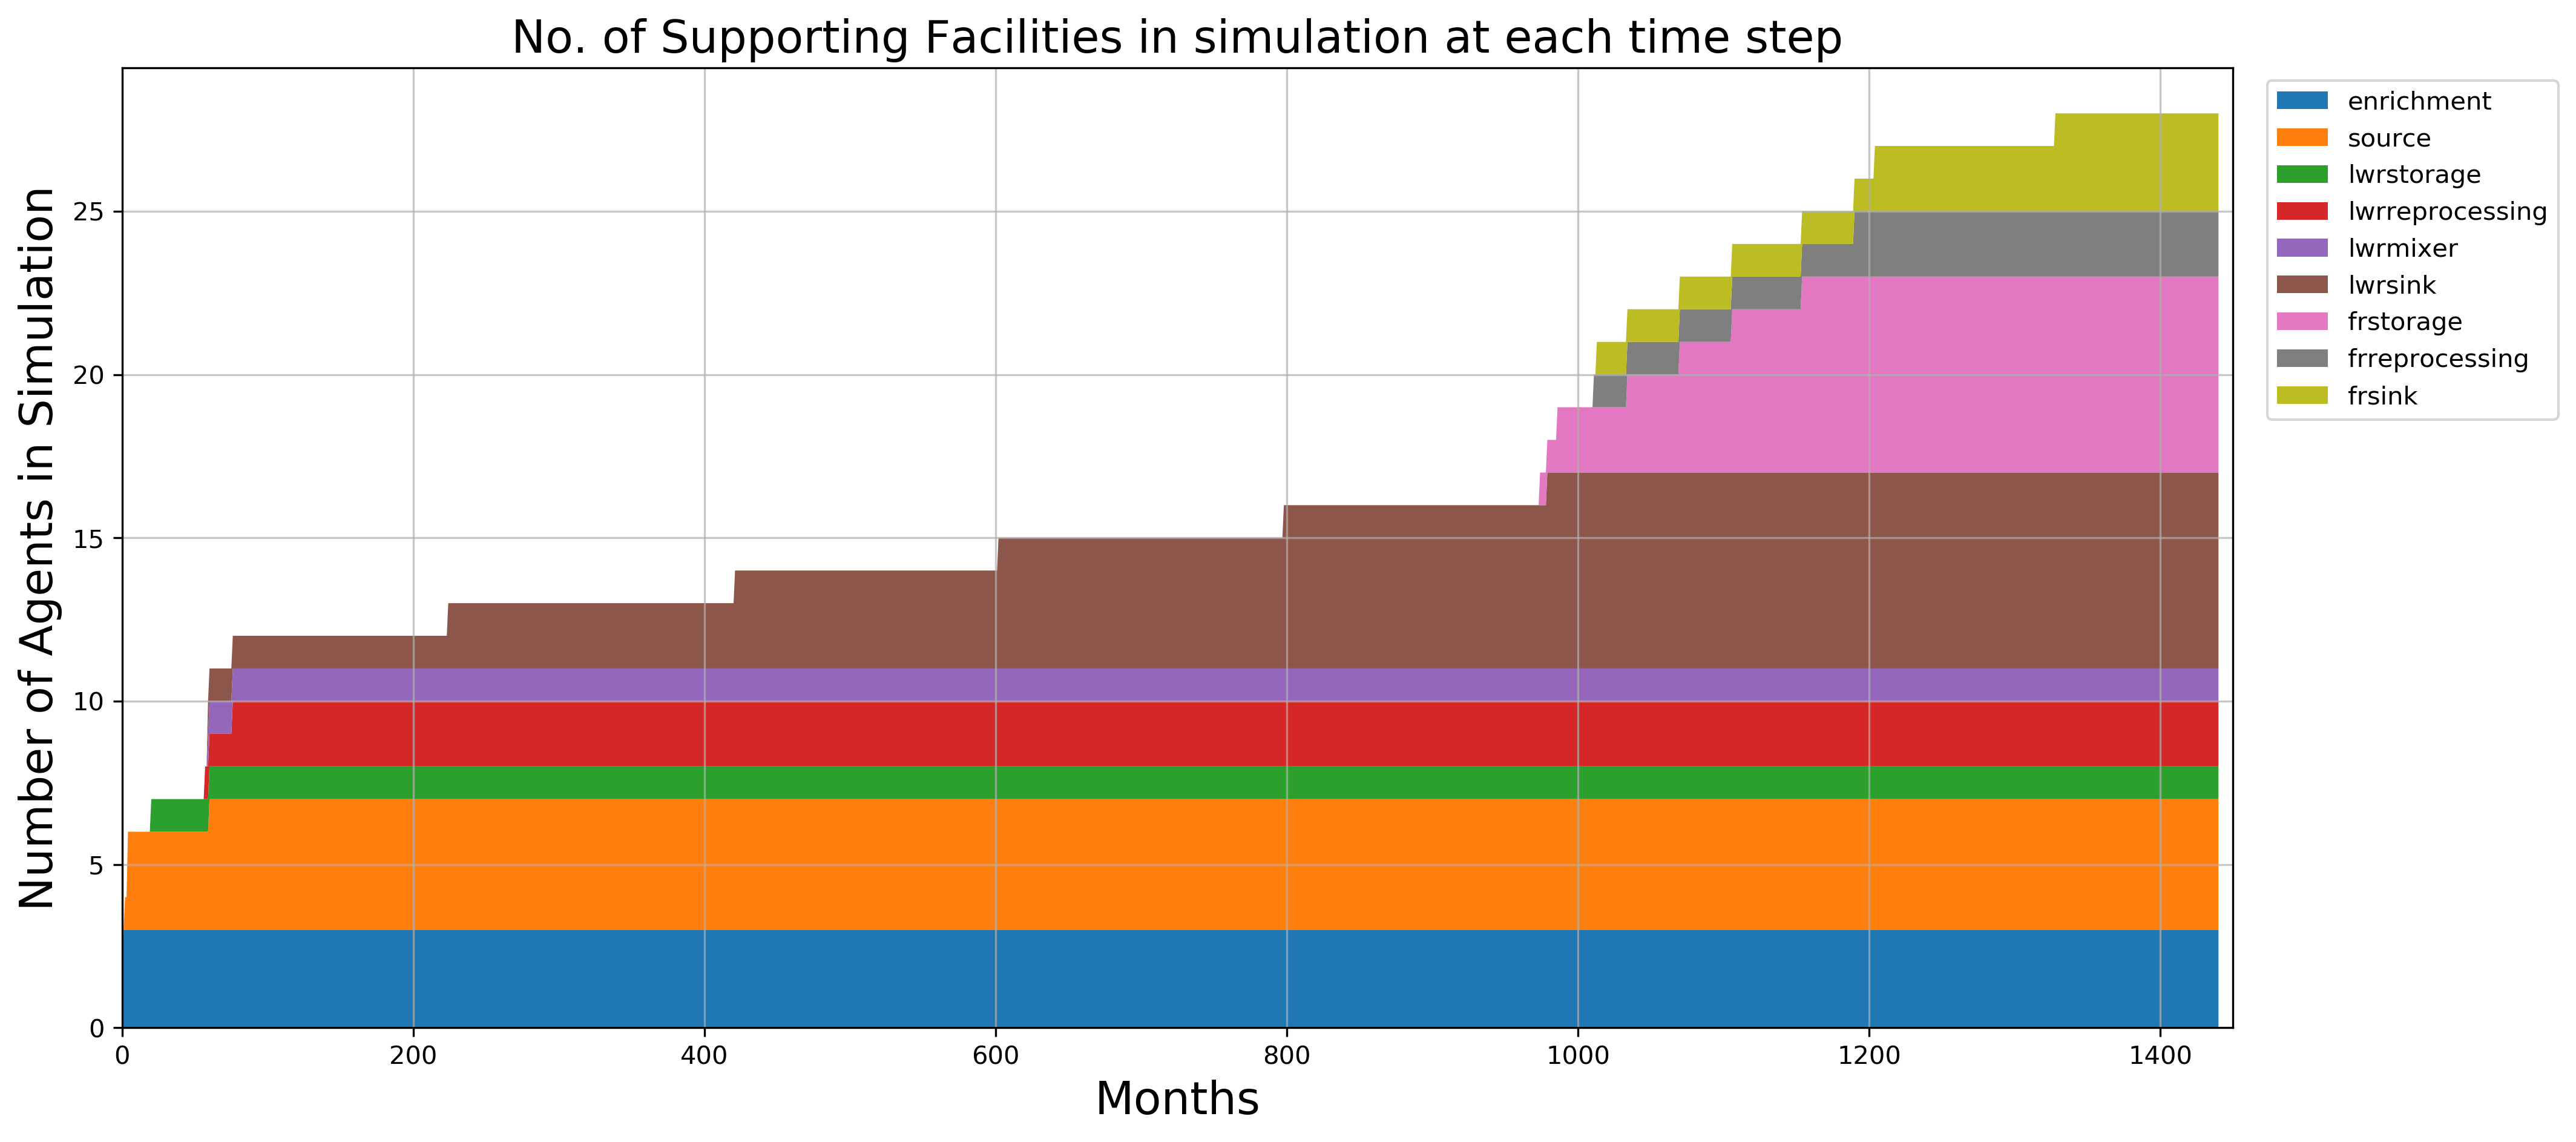
\includegraphics[width=\linewidth]{eg23-stack_support.png} 
		\caption{EG01-23: Supporting Facility Deployment}
		\label{fig:23support}
	\end{subfigure}
	\hfill
	\caption{Time dependent deployment of reactor and supporting facilities in 
	the EG01-23 constant power demand transition scenario. 
	\deploy automatically deploys reactor and supporting facilities 
	to setup a supply chain to meet constant power demand of $60000$ MW
	during a transition from \glspl{LWR} to \glspl{SFR}. }
	\label{fig:23stack}
\end{figure}

\begin{figure}[]
	\centering
	\begin{subfigure}[t]{1.2\textwidth}
		\centering
		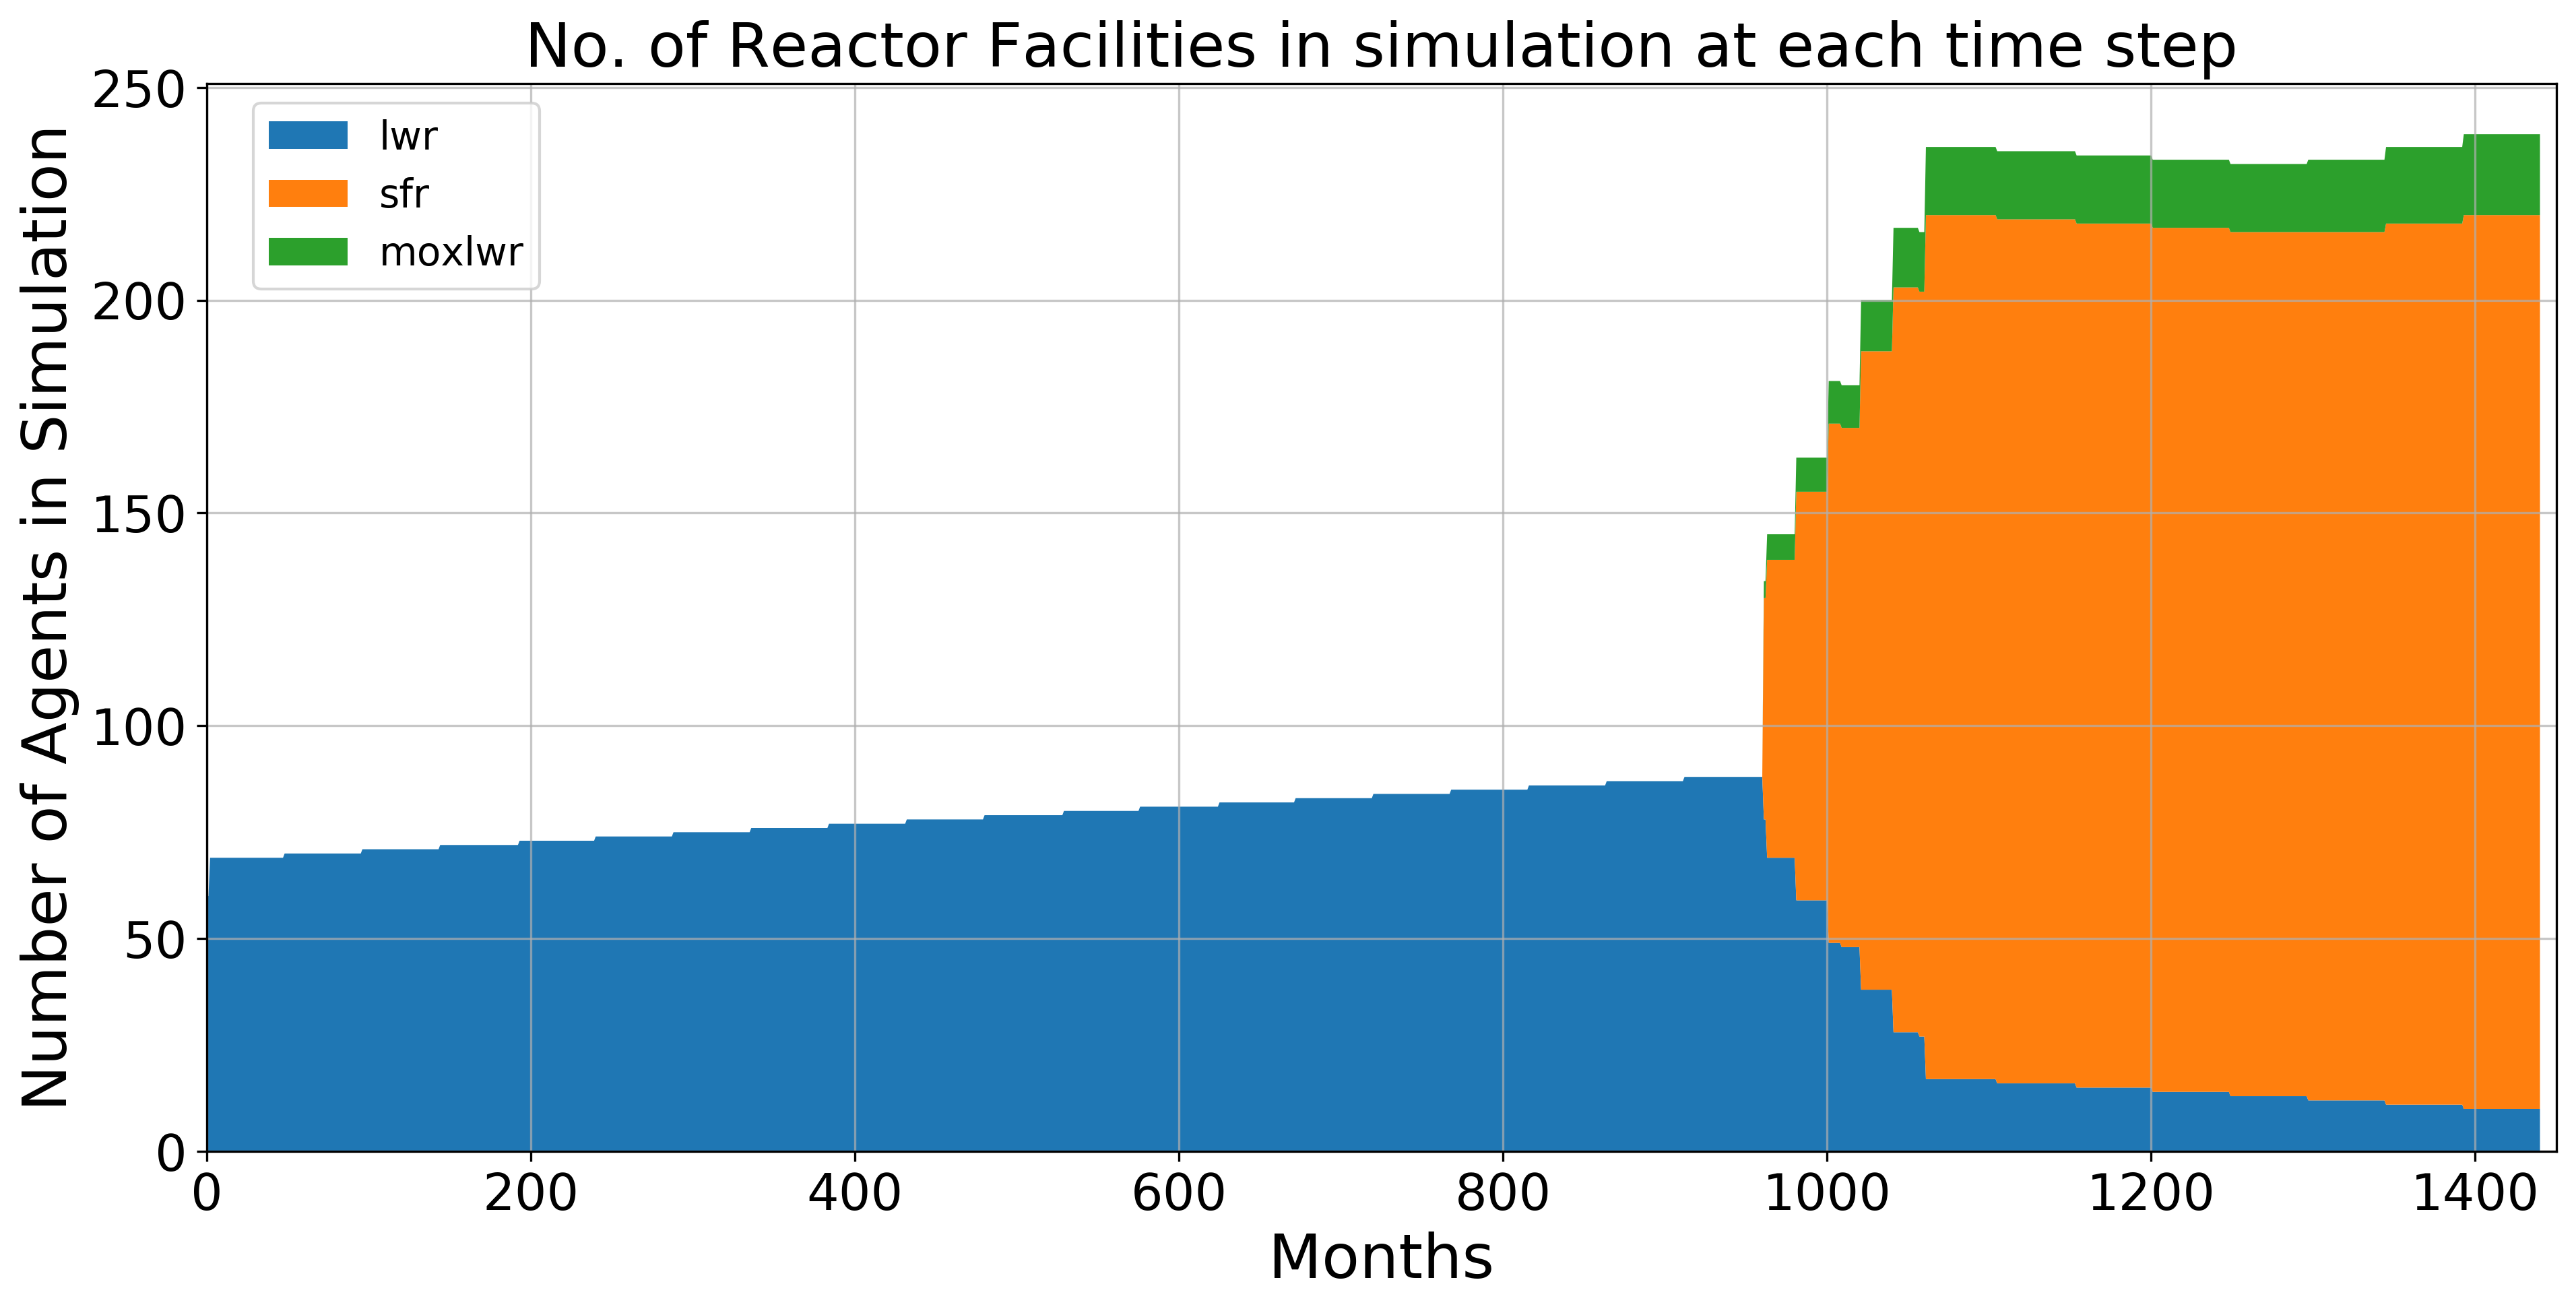
\includegraphics[width=\linewidth]{eg30-stack_reactor.png} 
		\caption{EG01-30: Reactor Deployment}
		\label{fig:30reactor}
	\end{subfigure}
	\vspace{1cm}
	\begin{subfigure}[t]{1.2\textwidth}
		\centering
		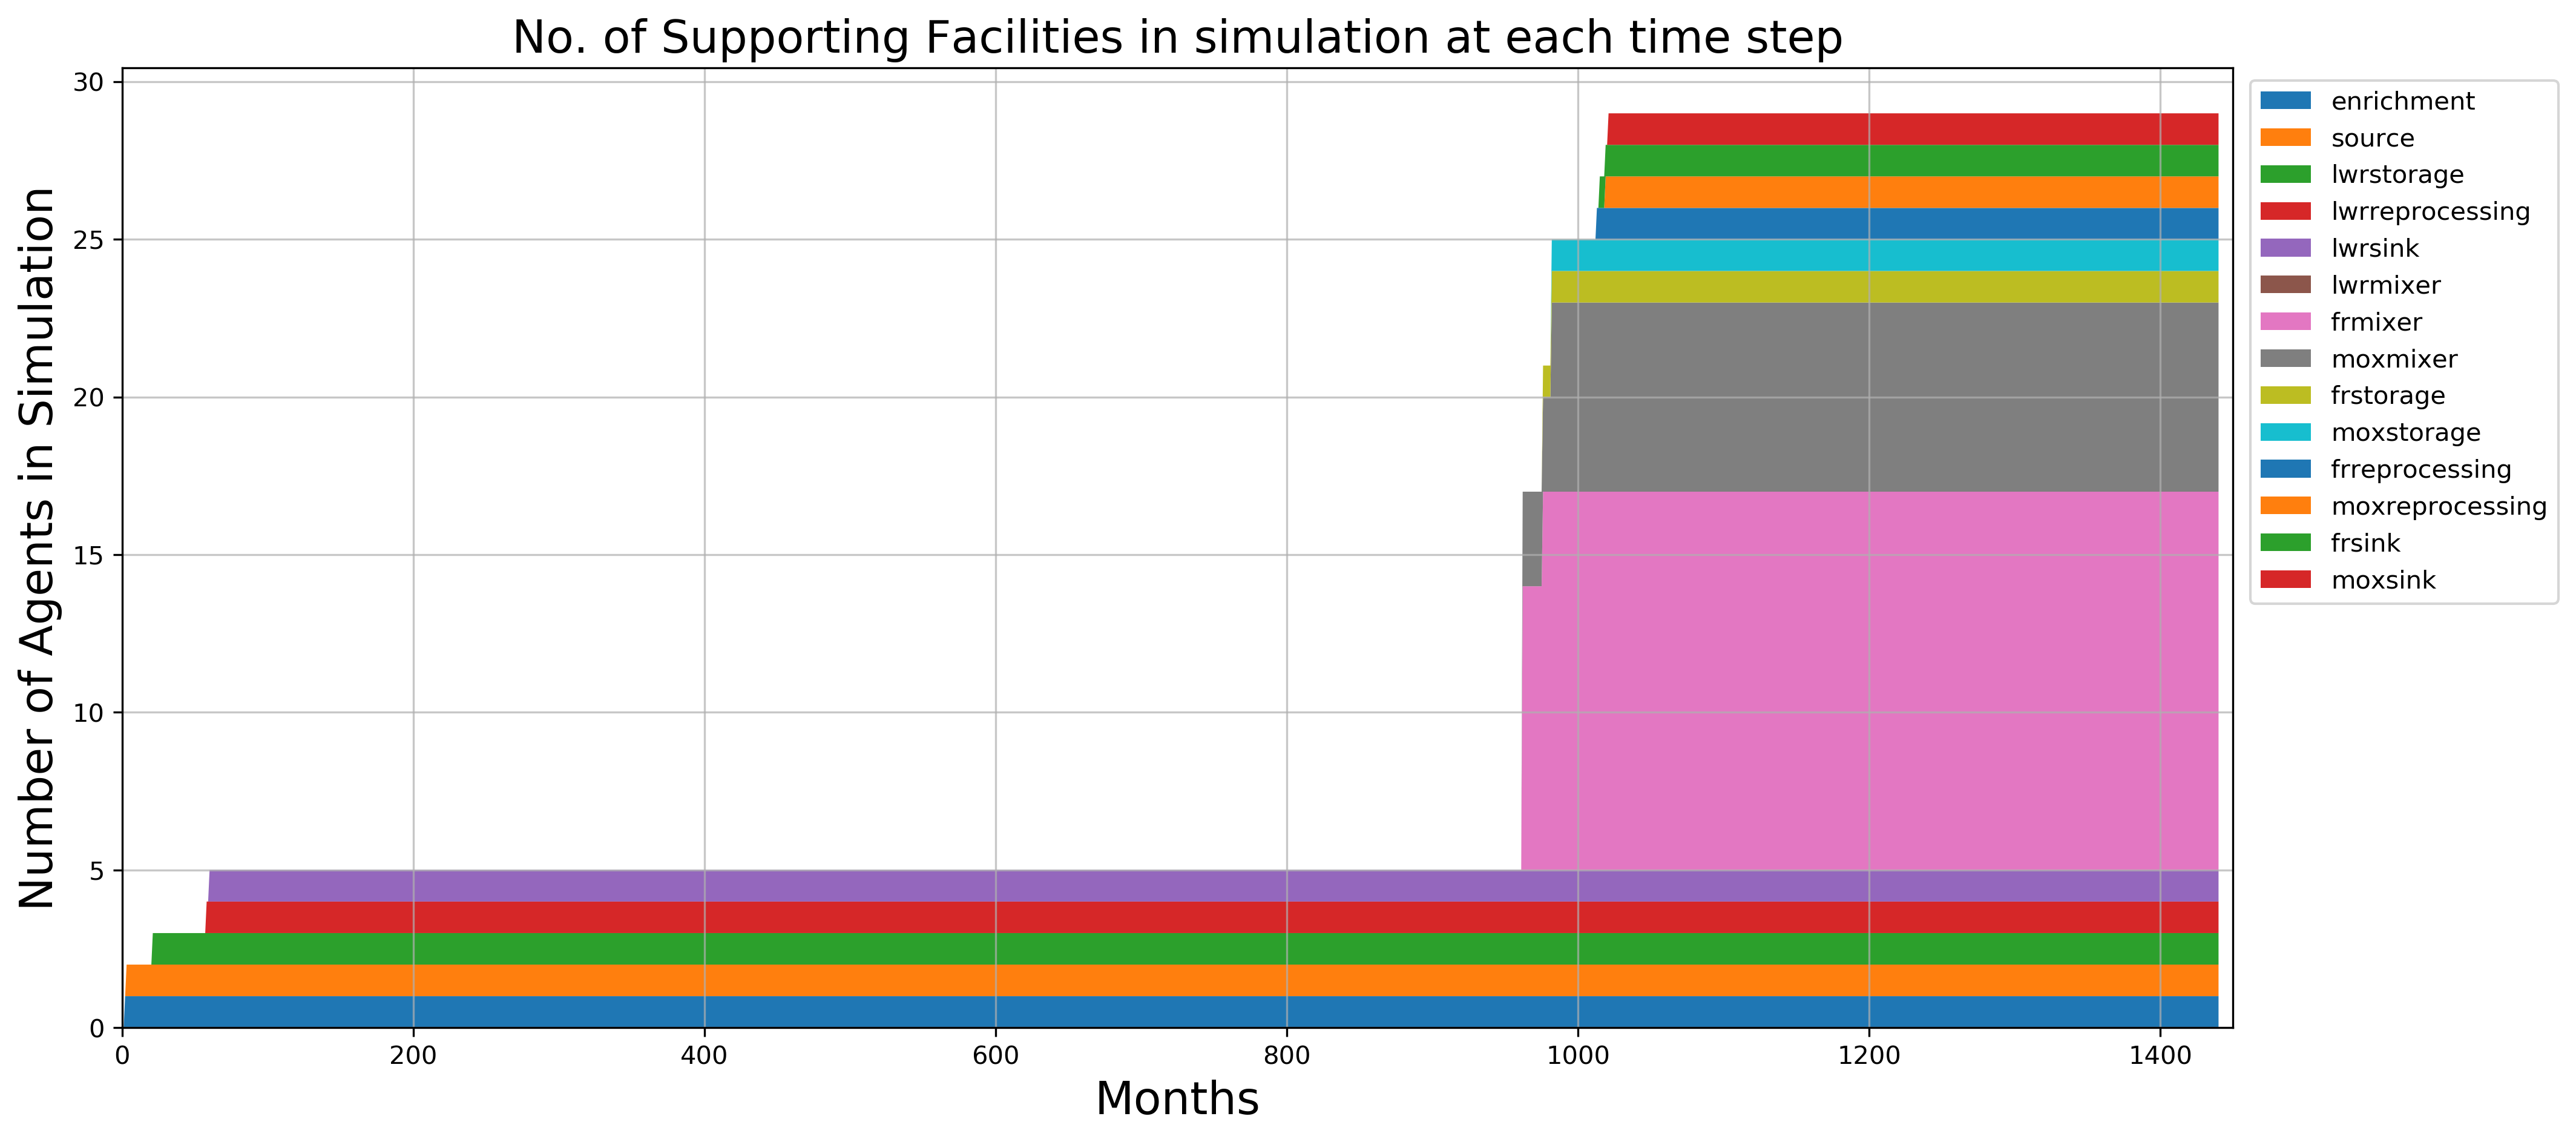
\includegraphics[width=\linewidth]{eg30-stack_support.png} 
		\caption{EG01-30: Supporting Facility Deployment}
		\label{fig:30support}
	\end{subfigure}
	\hfill
	\caption{Time dependent deployment of reactor and supporting facilities in 
	the EG01-30 linearly increasing power demand transition scenario. 
	\deploy automatically deploys reactor and supporting facilities 
	to setup a supply chain to meet constant power demand of $60000 + 250t/12$ MW
	during a transition from \glspl{LWR} to MOX LWRs and \glspl{SFR}. }
	\label{fig:30stack}
\end{figure}

\begin{table}[]
	\centering
        \caption{Undersupply/capacity of commodities for the best performing EG01-EG23,24,29,30 transition scenarios.}
		\label{tab:all-power}
		\footnotesize
        \begin{tabularx}{\textwidth}{l|RRRR}
		\hline
		& \multicolumn{3}{|c}{\textbf{Undersupplied Time Steps}} \\ \hline
		\textbf{Transition Scenario} & EG01-EG23 & 
		EG01-EG24 & EG01-EG29 & 
		EG01-EG30 \\ 
		\textbf{Power Demand} &Constant&Linearly Increasing&Constant&Linearly Increasing \\
		\textbf{Prediction Method} &\texttt{poly}&\texttt{fft}&\texttt{poly}& \texttt{fft}\\
		\textbf{Power Supply Buffer [MW]} &0&6000&0&8000 \\ \hline
		\textbf{Commodities} \\ 
		Natural Uranium		    & 2 	& 3  &  1  & 1 \\ 
		\gls{LWR} Fuel     	    & 4 	& 6  &  1  & 2\\ 
		\gls{SFR} Fuel     	    &  0 	& 0  &  2  & 2\\ 
		\gls{MOX} \gls{LWR} Fuel &-&-&2&2 \\
		Power      				&  6 	& 7  &  4 &  5\\ 
		\gls{LWR} Spent Fuel	& 1 	& 1  & 1 & 1\\ 
		\gls{SFR} Spent Fuel     	    &  1 	& 1  &  1  & 1\\ 
		\gls{MOX} \gls{LWR} Spent Fuel &-&-&1&1 \\ \hline 
	\end{tabularx}
\end{table}
